\documentclass[]{msulabm}
\usepackage[utf8]{inputenc}
\usepackage{amsmath}
\usepackage{graphicx}
%\usepackage[linktocpage]{hyperref}  % if not using colorlinks, use linktocpage
\usepackage[colorlinks]{hyperref}  % if not using colorlinks, use linktocpage
\usepackage{bm}            % bold math
\usepackage{multirow}
\usepackage[table]{xcolor} % provide alternating rows with colors
\usepackage{textcomp}
\usepackage{xfrac} % gives split-level fractions with '\sfrac{a}{b}
\usepackage{multicol}
\usepackage[section]{placeins} % provides \FloatBarrier, to keep floats from crossing this barrier
\usepackage{amssymb}
\usepackage{wrapfig} % provides wrapping figures with text.
%\usepackage{enumitem} % gives \begin{enumerate}[resume] to resume counting from previous enumerate
%\usepackage{subfigure}
%\usepackage{tikz} % to draw arrows
\usepackage{xtab} % provides xtabular, tabular environment that spans multiple pages and other awesome things
\usepackage[style=phys,biblabel=brackets,pageranges=false]{biblatex}
\usepackage{pdflscape}
\usepackage{ragged2e}
\usepackage{longtable}
\usepackage{mathabx} % gives astronomy symbols like \Earth
\usepackage{pdfpages}

\bibliography{references-manual,bbarker-zotero}

\newcommand{\abs}[1]{\left\lvert#1\right\rvert}

\title{Laboratory Manual}
\author{PHSC 12600 Matter, Energy, Space, \& Time \\ \\ The University of Chicago}
\date{Autumn 2020}

\pagestyle{ruled}

\definecolor{lgray}{rgb}{.2,.2,.2}

\makeevenfoot{ruled}{\thepage}{\footnotesize{\textit{Last updated \today}}}{}
%\makeevenfoot{ruled}{\thepage}{}}{}
\makeoddfoot{ruled}{}{\color{lgray} \tiny{This work is licensed under \href{http://creativecommons.org/licenses/by-sa/4.0/}{CC BY-SA 4.0} by \href{mailto:bbarker@uchicago.edu}{the University of Chicago}.}}{\thepage}


% allows us to use subcaptions from the memoir class in figures. See Memoir Section 10.9
\newsubfloat{figure}

% don't worry so much about filling every page.
%\raggedbottom

% raise the penalty for splitting footnotes across different pages. Default is 100.
\interfootnotelinepenalty=10000

%\includeonly{amplifier/amplifier} 

% creates a standard length to use 
\newlength{\answerskip}
%\setlength{\answerskip}{90pt} 

%% use plus / minus if latex is squeezing the answer space too much
\setlength{\answerskip}{2cm plus 0.2cm minus 0.2cm}

\newlength{\qaskip}
\setlength{\qaskip}{\answerskip}
\addtolength{\qaskip}{\baselineskip}

% reduce vertical space between chapters in table of contents. Default is 2em.
\setlength{\cftbeforechapterskip}{1em}

% allow for extra line on a page to help prevent widow/orphan lines.
\sloppybottom

% Now we can caption a table outside of the table float environment (good for multi-page tables)
\newfixedcaption{\freetabcaption}{table}

%\includeonly{snells-law/snells-law}
%\includeonly{ohms-law/ohms-law}

\begin{document}
\maxtocdepth{chapter}

 % start roman numbering
 \frontmatter

\maketitle

%\clearpage

%Brent W. Barker

%Department of Astronomy \& Astrophysics

%The University of Chicago

%5640 South Ellis Ave.

%Chicago, IL 60637

%\href{mailto:bbarker@uchicago.edu}{bbarker@uchicago.edu}

%\vspace{2\baselineskip}

%\includegraphics{cc-by-sa-88x31}

%\textcopyright{} 2018 Brent W. Barker. Except where otherwise noted, this work is copyrighted under the Creative Commons Attribution-ShareAlike International 4.0 License. To view a copy of this license, visit \url{http://creativecommons.org/licenses/by-sa/4.0/}.

%\vspace{\baselineskip}

%These labs, excluding "Impulse and Momentum" and the appendices, are a derivative of "\href{https://%sites.google.com/site/scientificabilities/ISLE-labs}{ISLE Labs}" by the Rutgers Physics and Astronomy %Education Research group, used under the Creative Commons Attribution International 4.0 License.
%To view a copy of this license, visit \url{http://creativecommons.org/licenses/by/4.0/}.

%At Rutgers University, many people contributed to this project over the years.
%The list of names is very long and includes: Eugenia Etkina, Alan Van Heuvelen, Suzanne Brahmia, David %Brookes, Michael Gentile, Anna Karelina, Michael Lawrence, Marina Milner-Bolotin, Sahana Murthy, Maria %Ruibal-Villasenor, Aaron Warren, Xueli Zou.

 % skip to next right leaf (``recto'')
 \cleartorecto

 % the star means that the ToC itself is not listed in the ToC
 \tableofcontents*

 % start arabic numbering
\mainmatter 

\chapter{Force and Motion 1}

\section{Learning Goals}

\begin{enumerate}
	\item Frame your work in terms of the scientific cycle described.
	
	\item Reflect on how your team worked together.
	
	\item Observe, record, and represent different types of motion.
	
	\item Develop a qualitative rule relating an object's change in motion to the unbalanced force exerted on it by other objects.
	
	\item Represent your ideas in multiple ways to help understand what you are trying to describe.
\end{enumerate}

\section{The Scientific Cycle\protect\footnote{adapted from \cite{etkina_college_2014}}}

One way of describing science is the process of incrementally improving a shared model of how our universe works. In different fields of science, different methods and cycles are used, so there is no ``One True Scientific Method.'' One can still create a model for the process of science, and we describe here one such cycle, summarized in Figure~\ref{me:fig:isle}.

In this cycle, there are three types of experiments, each one representing a different stage of the scientific effort. One stage, often started when encountering a novel phenomenon, is the \textbf{observational experiment}. This is an experiment that consists of deciding what to observe and how to observe it, collecting data, finding a pattern, and brainstorming possible explanations for what is observed (also called ``hypotheses'').

Once one has some trial explanations, one can test one or more of those with a \textbf{testing experiment}. Here, one designs a new experimental procedure and uses each hypothesis to predict what will happen. Then the prediction is compared to the procedure's outcome. If they are different, then the hypothesis is judged to be not a helpful explanation for that phenomenon. If they are the same, then it is still helpful. Throughout this stage, one may make various assumptions that would need to be validated, as they can effect the prediction or outcome.

Once a hypothesis has been tested enough for people to find it useful, then it can be applied to solve practical problems, or to determine properties of particular situations, in an ``application experiment.''

\begin{figure}
	\centering
	\includegraphics[width=0.7\textwidth]{force-motion-1/islegraphic.png}
	\caption{A model of the process some scientists go through to create knowledge.\cite{etkina_millikan_2015}}\label{me:fig:isle}
\end{figure}

\section{Team roles}

\textbf{Decide on roles} for each group member. The available roles are:

\begin{itemize}
	\item Facilitator: ensures time and group focus are efficiently used
	\item Scribe: ensures work is recorded
	\item Technician: oversees apparatus assembly, usage
	\item Skeptic: ensures group is questioning itself
\end{itemize}

these roles can (will?) rotate each lab, and you will report at the end of the lab report on how it went for each role. If you have fewer than 4 people in your group, then some members will be holding more than one role.

\section{Observation Experiment: Recording and Representing Motion}\label{fm1:sec:obs}

\textbf{Goal:} Record the motion of an object and represent its motion using a motion diagram.

\begin{steps}
	\item go to \url{https://physics.bu.edu/~duffy/HTML5/motion_diagrams.html}
	
	\item click play, watch Cars 1 and 2 (represented by the top (red) and bottom (blue) big dots) drive forward.
	
	\item notice that every second, a small dot is drawn to show where the car was at that time. this creates a visual record of the car's motion.
	
	\item How would you classify the object’s motion: motion with constant rate, increasing rate, decreasing rate? Explain how you decided.
	
	\item increase velocity of second car by dragging the velocity slider to the right.
	
	\item record how the motion diagram changes.
	
	\item imagine that you were given this plot without any velocity information - just the small dots. How could you tell which car was faster? Describe the procedure you would use to determine this.

	\item Observe the motion diagram captured in Figure\ \ref{fm1:fig:slowing}, specifically Car 2. How would you classify the object’s motion: motion with constant rate, increasing rate, decreasing rate? Explain how you decided.
	
%	\item Write a procedure to calculate how 
\end{steps}

\begin{figure}
	\centering
	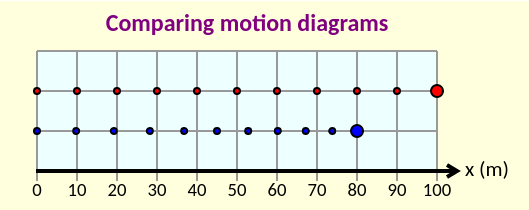
\includegraphics[width=0.6\textwidth]{force-motion-1/motion-diagrams-slowing.png}
	\caption{Motion diagrams of Car 1 (red, top) and Car 2 (blue, bottom). The small dots were marked every 1 second during the cars' motions.}\label{fm1:fig:slowing}
\end{figure}

%\begin{figure}
%	\centering
%	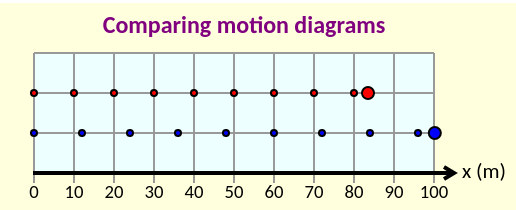
\includegraphics[width=0.5\textwidth]{force-motion-1/motion-diagrams.png}
%	\caption{Motion diagrams of Car 1 (red, top) and Car 2 (blue, bottom). The small dots were marked every 1 second during the cars' motions.}
%\end{figure}

\section{Observation Experiment: Forces Exerted on an Object by	Other Objects}

\textbf{Goal:} Learn to represent forces exerted on an object by other objects in a clear and efficient way.

\textbf{Available Equipment:} Two household objects of different weights and similar shapes, for example a bowling ball and a tennis ball.

Pick up a tennis ball and hold it stationary in your hand. Then pick up a bowling ball and hold it the same way. Do you feel any difference? Now we will learn to represent this difference graphically using force diagrams (sometimes called free-body diagrams).

\textbf{For each situation (tennis ball and bowling ball) do the following:}
\begin{steps}
	\item List all the objects that interact with the ball.  The ball is called the "object of interest" since that's what we are focusing our attention on.  To interact with the ball, most other objects need to be in physical contact with it (the Earth is an exception --- it can interact gravitationally from a distance).
	%Explain how you can represent these interactions on a diagram so that Alex can understand them.
	
	\item Represent the ball with a dot and use an arrow to represent each interaction of another object with the ball. Connect the tails of the arrows to the dot. Label each force arrow with an $\vec{F}$ that has two subscripts. The first subscript represents the object that exerts the force on the object of interest; the second subscript represents the object of interest itself. For example, the force that the hand exerts on the ball can be written as $\vec{F}_{H \rightarrow B}$. Pay attention to the lengths of the arrows on each force diagram.  Should any of them be longer or shorter than others?
	
	\item Indicate what forces "cancel" or "balance" each other. Indicate if there is an "unbalanced" force. Explain how your force diagram is a better way of describing the forces being exerted on an object than written words.
	
	\item Why are forces represented by arrows and not just by numbers or lines?
	
	\item You can compare your force diagram to the one found at \url{https://physics.bu.edu/~duffy/HTML5/force_motion_1D.html} . Notice how the diagram changes when you change the mass.
\end{steps}

\section{Testing Experiment: Does an object’s motion always	occur in the direction of the unbalanced force exerted on it by other objects?}

\textbf{Goal:} Test two ideas (also called \textit{hypotheses}):
\begin{enumerate}[label=(\alph*)]
	\item An object always moves in the direction of the unbalanced force exerted on it by other objects.
	\item An object always changes its motion in the direction of the unbalanced force exerted on it by other objects.
\end{enumerate}

\textbf{Available equipment:} Everything around you. You might be helped by things that roll, and forming a ramp with books. Also the following simulation: \url{https://phet.colorado.edu/sims/html/forces-and-motion-basics/latest/forces-and-motion-basics_en.html} (try the Motion screen in particular)

\begin{framed}
	\textbf{Self-assessment:} To help you improve your scientific abilities, we provide you with self-assessment rubrics.
	A rubric is a method of aligning expectations for performance.
	Self-assessment is determining how well you performed a particular task.
	So, these self-assessment rubrics are designed to help you evaluate your performance while you are designing and performing your experiment.
	
	The complete set of rubrics is available in Appendix~\ref{cha:rubrics}.
		In each lab, your report will be assessed using Rubric F, found in Table~\ref{rubric:f}, as well as 5 additional rubric rows listed in that lab.
		Each week, read through these and use them to evaluate your work as you design and perform the experiment.
		Your instructor will use the same rubrics to determine part of your grade for the lab. In particular, each row will be worth 3 possible points (from ``Missing'' being 0 points to ``Adequate'' being 3 points).
\end{framed}

\textbf{Rubrics to focus on during this experiment:} C1, C2, C4, C7, C8. See Table~\ref{rubric:c} for details.

\begin{steps}
	\item First, think about the two competing ideas that you are testing. Think about how you can use the available equipment to design experiments relevant to both of them. Also, think what the words "test an idea" mean in real life. Does "testing" mean trying to support an idea or trying to disprove an idea? Which approach do you think is more productive? When you come up with at least 2 possible experiments, \textbf{contact an instructor or TA} and discuss your experiments with them.
	
	\item After your discussion with the TA, record the two experiments you are going to perform. Draw pictures and force diagrams for each situation.
	
	\item Make a prediction of the outcome of each experiment if idea (a) were correct.
	
	\item Make a prediction of the outcome of each experiment if idea (b) were correct.
	
	\item Make a table to record the following information for the object: (1) the direction of the motion, (2) the direction of the change in motion, and (3) the direction of the unbalanced force.
	
	\item Perform each experiment and record the outcome in the table.
	
	\item Decide if any of the predictions are consistent with the outcomes of the experiments.
	
	\item Make a judgment about each idea.  That is, decide which, if any, of the ideas are consistent with the outcome of the experiment. Remember, the goal of a testing experiment is to \textbf{disprove} ideas, not to support them.
	
	\item Include arguments for why your judgments are reasonable in your report.
	
	\item The experiment in Section \ref{fm1:sec:obs} was called an observational experiment, and the experiment in this section was called a testing experiment. How do these names reflect the differences in performing these two kinds of experiments? (What aspects does one kind have that the other type does not?)
	
	\item Design, describe, and (if possible) perform two more experiments in which the object does not move in the direction of the unbalanced force. Draw a motion diagram and a force diagram for each experiment.
	
	\item You have represented motion and forces in different ways.  Explain how these representations helped you to find a pattern/relationship between motion and forces.
\end{steps}

\section{Why Did We Do This Lab?}

\begin{steps}
	\item In a paragraph, summarize what you have learned during this first lab in terms of physics content and in terms of the purpose of the two kinds of experiments you designed and performed.
	
	\item Describe how your understanding of the relationship between force and motion is different from your understanding before.
\end{steps}

\section{Group dynamics}

\begin{steps}
	\item Write a 100--200 word reflection on group dynamics and feedback on the lab manual. Address the following topics: who did what in the lab, how did you work together, what successes and challenges in group functioning did you have, and what would you keep and change about the lab write-up?
	
	\item Write a paragraph reporting back from each of the four roles: facilitator, scribe, technician, skeptic. Where did you see each function happening during this lab, and where did you see gaps?
\end{steps}

\section{Report checklist and grading}

The lab grade consists of 3 points for each of seven scientific ability rubric rows (the 5 listed above, which apply just to that section, as well as F1 and F2, applied to the entire report), and 9 points for providing evidence in the lab report of completing all steps of the lab, including answering every question, for a total of 30 points.
\chapter{One-dimensional kinematics}

\section{Learning goals}

\begin{enumerate}
 \item Represent the motion of an object graphically, verbally, and mathematically. Change representations as required to describe your observations effectively.
 
 \item Apply kinematics ideas to solve a practical problem.
 
 \item Estimate experimental uncertainties in order to make judgments about experimental results.
\end{enumerate}

\section{Lab Team Roles}

Decide which team members will hold each role this week: facilitator, scribe, technician, skeptic.

\section{Observation Exp: Observe and represent motion}

\textbf{Goal:} Represent the motion of an object graphically, translate between graphical and verbal representations, and change position, velocity, and acceleration consistent with those representations. This focuses on the part of the observation experiment that involves recording data.

\textbf{Available equipment:} Simulation found at \url{https://physics.bu.edu/~duffy/HTML5/1Dmotion_graph_matching.html}

\begin{steps}
	\item Open the simulation at the address listed above. Notice that there is a position vs. time graph, a velocity vs. time graph, and a motion diagram.
	
	\item For the following different situations, imagine that you are wearing a motion sensor and it will make a motion diagram as you walk, marking your position every second. For each way of walking described, adjust the initial position, velocity, and acceleration sliders to create the motion diagram that it would create. Each way of recording your observations is called a "representation". Construct an organized table similar to the one in Table\ \ref{1dk:tab:reps} to record different representations.
	
	\begin{table}
		\begin{tabular}{p{.3\textwidth}|p{.3\textwidth}|p{.3\textwidth}}
			\textbf{verbal description of experiment} & \textbf{motion diagram} & \textbf{graphs} \\
			\hline
			Include where you start and end your motion, how you moved, and the time interval for which you moved & Remember to include dots and the number line. & position-vs-time and velocity-vs-time
		\end{tabular}
		
		\caption{Format for table of representations.}\label{1dk:tab:reps}
		
	\end{table}
	
	Try the following four experiments:
	
	\begin{enumerate}
		\item Stand still, then walk forward at a steady pace, then stand still again.
		
		\item Walk backward at a steady pace.
		
		\item Walk forward at a steady pace for 4 seconds, then walk steadily but at a faster pace backward for the next 2 seconds.
		
		\item Walk forward at a steady pace for 2 seconds, then continually increase your speed.
	\end{enumerate}
	
	\item A fellow student, Alex, does not understand why it is a good idea to represent the same information in these three different ways (verbal, motion diagrams, graphs). What do you say to Alex to help them understand the use in doing this?
	
	\item What was the purpose of this first experiment? Specifically what did you learn? How did you learn it?
	
\end{steps}

\section{Testing exp: Do you understand graphs?}

\textbf{Goal:} Adjust the simulation parameters in such a way that the graphs produced by your imagined motion match a few pre-determined graphs.

\textbf{Available equipment:} Simulation found at \url{https://physics.bu.edu/~duffy/HTML5/1Dmotion_graph_matching.html} 

\begin{steps}
	
	\item Open the simulation at the address listed above. Notice the buttons for Graph 1 through Graph 10.
	
	\item Pick three of the position graphs (Graphs 1--5) and three of the velocity graphs (Graphs 6--10) to match.
	
	\item Do the following for each:
	\begin{enumerate}
		\item Before you proceed to perform the experiment, you need to decide how you will move the sliders. Predict, based on your observations from the first experiment and your knowledge of kinematics, how you should move to produce graphs that match those that are on the screen. \textbf{Record your predictions.}
		
		\item After you have made your prediction, perform the experiment by adjusting the position, velocity, and acceleration sliders and using the play and pause buttons. \textbf{Record the outcome graph.}
		
		\item If the graph produced by your motion did not match the provided graphs, \textbf{discuss in your report} possible reasons and how you would move differently to make the motion match the graph more closely.
		
		\item Where on the graph is the position of the object represented?  Where is the time represented?
	\end{enumerate}
	
	\item How do motions that are represented by $x(t)$ lines with various slopes differ from each other? What information can we obtain from the slope of an $x(t)$ graph?
	
\end{steps}

\section{Application experiment: how long is the brick?}

\begin{itemize}
	\item \textbf{Goal:} Determine the length of a brick in a mechanics simulation.

	\item \textbf{Available equipment:} Stopwatch (app, website, watch, etc.), simulation at \url{https://phet.colorado.edu/sims/html/forces-and-motion-basics/latest/forces-and-motion-basics_en.html}

	\item \textbf{Rubrics to focus on:} D2, D4, G1, G2, G4
	
	\item Since this is the first application experiment we've done, read through the application experiment rubric, D. Rubric G is also important, as it is about data analysis, and this is a quantitative experiment.
	
	\item For comparing two values with uncertainties, to see if they are the ``same'' or not, see Appendix~\ref{unc:sec:comparing}.
\end{itemize}

\begin{steps}
	\item Open the simulation in the link above and go to the section marked "Motion". Notice that you can select different view options in the upper right hand corner.
	
	\item Brainstorm two \textit{independent} experiments to determine the length of the brick. One of the ways must use the formula that describes the relationship between displacement $\Delta x$, velocity $v$, and time $t$ during constant velocity,
\begin{equation}
	 \Delta x = v t \,.
\end{equation}
	
	Another way could involve the typical size of other objects in the simulation.
	
	\item When you come up with at least 2 possible experiments, \textbf{contact an instructor or TA} and discuss your experiments with them.
	
	\item For each experiment you conduct, including the following in your report:
	
	\begin{enumerate}
		\item Describe your experimental procedure. Include a sketch of your experimental design.
		
		\item List the sources of experimental uncertainty.
		
		\item Explain what steps you will take to minimize experimental uncertainty.
		
		\item Perform the experiment. Record the data using appropriate representations (motion diagrams, tables, graphs, etc.). Determine the uncertainty in the measurements you made (you will need to do multiple trials to do this).
		
		\item Use your measurements and their uncertainties to determine the length of the brick. Propagate uncertainties through your calculations as described in Appendix~\ref{unc:sec:prop}.
		
		\item Report your result as a value plus or minus the uncertainty (e.g. $5 \pm 1$ m).
	\end{enumerate}

	\item Compare the two values you obtained for the brick length using the method described in Appendix~\ref{unc:sec:comparing} and obtain a $t'$ value.
	
	\item Taking into account experimental uncertainties and the assumptions you made, decide if these two values are consistent or not. If they are not consistent, explain possible reasons for how this could have happened (for example, assumptions made, underestimating uncertainty).
	
	\item Decide on a final value (including uncertainty of that value) for the brick length based on the results of your experiments.

	\item Describe the shortcomings you noticed in the experiments. Suggest specific improvements.
	
\end{steps}

\section{Why did we do this lab?}

\begin{steps}
	\item Explain how each of the group member's understanding of representations of motion is different now compared to before the lab.
	
	\item In this lab you conducted an observation experiment and an application experiment. How are the purposes of an observation experiment and an application experiment different?
	
	\item In your own words, what is it meant by "experimental uncertainty"?  Why should we care about it?
	
	\item Give real-life examples of instances when people need to collect and analyze quantitative data (numbers with units) to describe and understand what is happening.
\end{steps}

\section{Group dynamics}

\begin{steps}
	\item Write a 100--200 word reflection on group dynamics and feedback on the lab manual. Address the following topics: who did what in the lab, how did you work together, what successes and challenges in group functioning did you have, and what would you keep and change about the lab write-up?
	
	\item Write a paragraph reporting back from each of the four roles: facilitator, scribe, technician, skeptic. Where did you see each function happening during this lab, and where did you see gaps?
\end{steps}

\section{Report checklist and grading}

The lab grade consists of 3 points for each of seven scientific ability rubric rows (the 5 listed above, which apply just to that section, as well as F1 and F2, applied to the entire report), and 9 points for providing evidence in the lab report of completing all steps of the lab, including answering every question, for a total of 30 points.
\chapter{Force and Motion 2}

\section{Learning Goals}

\begin{itemize}
	\item Make careful observations and find quantitative patterns.
	
	\item Choose and fit models to data in order to describe a pattern.
	
	\item Test a hypothesis quantitatively.

\end{itemize}

\section{Lab Team Roles}

Decide which team members will hold each role this week: facilitator, scribe, technician, skeptic. If there are three members, consider having the technician and skeptic roles be held by one person.

\section{Observation experiment: how fast and how far does force get you?}\label{fm2:sec:obs}

\textbf{Goal:} Your friend Taylor noticed that when they pushed on a skateboard, it started going faster. They started wondering --- how does force and mass affect how far an object goes and how fast it gets? Investigate this and find some quantitative patterns. Represent the patterns in graphical and formula form.

\textbf{Available equipment:} Force and Motion Basics simulation (\url{https://phet.colorado.edu/sims/html/forces-and-motion-basics/latest/forces-and-motion-basics_en.html})

\textbf{Rubric rows to focus on:} B1, B3, B5, B7, B8 (and F1 and F2 for all sections, like normal)

\begin{steps}
	\item read through the rubric B to see the steps to follow and what to ensure you include, given the rubric rows listed above.
	
	\item Taylor's description of what to look at might not be specific enough for you. They're not answering your texts about it, so you'll need to decide what specific phenomenon to investigate. Discuss and brainstorm experiments with your group (and play with the sim), then discuss with a TA or instructor. (There are several different phenomena you can choose. There is not a right one we are looking for)
	
	\item Design and record your experimental setup and procedure, including a diagram of the setup.
	
	\item What quantities are you measuring, in particular? And which are the independent and dependent variables?
	
	\item Describe in detail how you are making the measurements.
	
	\item Conduct your experiment and record your data. Express in a table or graph form.
	
	\item Identify a pattern in the data. Your resulting pattern should be described precisely in words, and in an equation that describes how the dependent variable changes in response to a change in the independent variable(s).
	
	\item You may find it useful in this experiment or future ones to fit a test function to data. This is called curve fitting. You can use your preferred curve fitting program, or use SciDaVis, a free open source graphical analysis program.
	
	\begin{itemize}
		\item You can download and install it on your computer from \url{https://sourceforge.net/projects/scidavis/}.
		%, or you can use the lab computers, which have it installed already.
		
		\begin{framed}
			\textbf{Mac users:} if you get an error when trying to run SciDaVis, saying that it is from an unidentified developer, follow the directions at the following website to let it run:
			
			\url{https://support.apple.com/guide/mac-help/open-a-mac-app-from-an-unidentified-developer-mh40616/10.15/mac/10.15}
		\end{framed}
		
		\item Optionally, watch the short video tutorial from the Lab Module on Canvas, describing how to enter data into SciDAVis and create a curve fit.
		
		\item In SciDAVis X is the independent variable and Y is the dependent variable.
		
		\item To plot the data, Highlight the data X,Y, and/or yEr you want to plot (by clicking the X column, holding the Ctrl key, then clicking the Y column).  Then click Plot $\Rightarrow$ Scatter. Clicking on the axis, curves, axis titles, or data points allows you to customize your graph.
		
		\item To fit an equation to the data, first enter the data, then save the project, so you won't accidentally lose your work. Then, select Analysis $\blacktriangleright$ Fit Wizard... from the drop-down menu. Type your desired equation into the large box. You can use any of the functions you can find in the lists at the top of the window and combine them how you would like. For fit parameters, use the letters a, b, c, and so on. For each fit parameter you use, include it in the list of parameters. For example, if you think the data are best represented by a tangent function, you could type ``\texttt{b*tan(c*x+d)}'' in the box. Then click the ``Fit $>>$'' button. A new screen will come up.  Enter your initial guesses for the parameters.  Also enter the high and low range for X. Then the ``Fit'' button to fit the data with this equation. This finds the parameters for the equation that make it best fit the data. The values for the fit and their uncertainties will be displayed in the Results log. Experiment to find an equation that seems to fit well.
	\end{itemize}
\end{steps}

\section{Testing experiment: displacement and time under constant acceleration}

\textbf{Goal:} Taylor performed their own observation experiment and arrived at the following mathematical description for the displacement $x$ of an object of mass $m$ subject to a constant force $F$ for a duration $t$, starting from rest:
\begin{equation}
 x = \frac{F t^2}{m} \,.
\end{equation}
Taylor would like you to verify this. I, the lab manual, would like to show you one way of using curve fitting to test it.

\textbf{Available equipment:} 
Force and Motion Basics simulation (\url{https://phet.colorado.edu/sims/html/forces-and-motion-basics/latest/forces-and-motion-basics_en.html})

\textbf{The idea} is to produce a number of $(t,x)$ data points from an object of known mass, subject to a constant force and plot them (time on the horizontal axis and displacement on the vertical axis). Then fit a quadratic function to those points, of the form $Y = C*X^2$. The curve fit will produce the best fit parameter $C \pm \delta C$. In this situation, the hypothesis predicts that $C = F/m$. Comparing the values using their uncertainties, the prediction will match the outcome if the $t'$ statistic is less than 1.

\begin{steps}
	\item Discuss what experimental procedure to use to collect the data using the sim. How many data points do you need? How will you determine the uncertainty of each data point? What will you use to take the measurements and what role will each person take in the experimental procedure? \textit{Hint: if things are happening too quickly to record, you can take a video and then pause as needed during playback.}
	
	\item Write down your procedure and draw a sketch to describe the setup.
	
	\item Conduct the data collection, including uncertainty estimation for each point.
	
	\item Execute the data analysis as described above. \textbf{Record the graph and best fit parameters with their uncertainties.}
	
	\item Calculate the $t'$ statistic and use it to decide if the outcome matches the prediction.
	
	\item Based on this experiment, what would you say to Taylor about their hypothesis?
\end{steps}

\section{Application experiment: mass of the mystery box}

\textbf{Goal:} Use the pattern you discovered in Section \ref{fm2:sec:obs} to find the mass of the mystery box in the Force and Motion Basics simulation.

\textbf{Available equipment:} 
Force and Motion Basics simulation (\url{https://phet.colorado.edu/sims/html/forces-and-motion-basics/latest/forces-and-motion-basics_en.html})

\begin{steps}
	\item Design and conduct the experiment. Include a description and sketch of the setup and procedure, data table, uncertainty analysis, and final determination of the box's mass.
	
	If you are unable to use the pattern you discovered to solve the problem, and your TA agrees, then you can use results from Newtonian mechanics, for example $F = ma$ and $a = \frac{v_f - v_i}{t}$ , where $a$ is the acceleration, $v_f$ is the final velocity, and $v_i$ is the initial velocity.
\end{steps}
\chapter{Energy Conservation}

\begin{itemize}
	\item intro energy conservation, types of energy
	
	\item intuitively derive $U=mgh$
\end{itemize}


\chapter{Is light a particle or a wave?}

You may have heard that light is both a particle and a wave, and that this is paradoxical. We want you to get a clear sense of why physicists have come to this wild conclusion, and continue to practice working with the scientific cycle that we have presented.

\section{Learning goals}

\begin{itemize}
	\item Make careful predictions based on hypotheses and a given experimental setup.
	
	\item Gain a clear sense of how light behaves like a particle, and how it behaves like a wave.
\end{itemize}

\section{Lab Team Roles}

Decide which team members will hold each role this week: facilitator, scribe, technician, skeptic. If there are three members, consider having the skeptic double with another role. Consider taking on a role you are less comfortable with, to gain experience and more comfort in that role.

Additionally, if you are finding the lab roles more restrictive than helpful, you can decide to co-hold some or all roles, or thinking of them more like functions that every team needs to carry out, and then reflecting on how the team executed each function.

\section{Observation experiment: describing waves and particles}

In order to make predictions in the testing experiments with light, it will be helpful to determine what properties waves and particles have in more obvious situations, so that these properties can be applied to less obvious situations with light.

\subsection{Goal}

Describe patterns of behavior of waves and particles that can be used to differentiate between them.

% target observations for particles:
% - when two of them travel to intersect, they collide and change direction
% - can only be emitted or absorbed as discrete units

% target observations for waves:
% - when two of them travel to intersect, they overlap and continue undisturbed
% - continuous transmission of energy


\subsection{Available equipment (simulated)}

\begin{itemize}
	\item Particle box: box where particles move towards each other and interact (Simulation:  \url{https://phet.colorado.edu/sims/html/collision-lab/latest/collision-lab_all.html} (Select ``Explore 2D''))

	\item Ripple tank: tank of shallow water with set of plungers (to create waves) and walls that obstruct the path of waves (Simulation: \url{http://www.falstad.com/ripple/})
	
	\item String attached to an oscillator (Simulation: \url{https://phet.colorado.edu/sims/html/wave-on-a-string/latest/wave-on-a-string_en.html})
\end{itemize}

\subsubsection{What happens when their paths intersect?}

%{\color{red} This might not have enough discovery about interference leading to dark fringes. This also might not have enough discovery that particles travel in straight lines while waves spread out like wavelets.}

\begin{steps}
	\item In the particle box, \textbf{observe and record} what happens when the two particles approach each other and interact. How are their motions different after the interaction?
	
	\item In the ripple tank, watch the wave crests (light color) expand away from the source, a plunger pushing down and up in the water.
	
	\item Click anywhere in the tank to touch your finger into the water momentarily and create a ripple (a single wave crest). \textbf{Observe and record} what happens when the ripple approaches each wave crest and interacts. How are the ripple and wave motions different after the interaction?

	\item Summarize the difference between particles and waves in this case.

\end{steps}

\subsubsection{How do they deliver energy?}

\begin{steps}
	\item With the wave on a string simulation, click ``loose end'' on the right side, then click and drag the wrench to see how it moves the string.
	
	\item Select ``Oscillate'' on the left side of the screen. Reduce the amplitude to about 0.2 cm. Reduce the frequency to exactly 1.47 Hz. Reduce the damping to ``None''.
	
	\item Press ``Restart'' to reset the string to neutral.
	
	\item Watch what happens as the wave delivers energy to the ring at the right. Does the wave deliver energy continuously or in short bursts? Is there a minimum amplitude needed to start the ring in motion?
	
	\item In contrast to this, consider the following example of particles: imagine that you have a bag of basketballs and a friend is sitting on a chair on wheels, which is resting on a carpet. If you toss the ball gently to them, they don't budge at all. But if you toss a ball fast enough, it pushes them back. Does this deliver energy continuously or in short bursts? And if you keep tossing balls gently to them, will that ever get them moving?

	\item Summarize the difference between particles and waves in this case.

\end{steps}

\section{Testing experiment: is light a particle or wave?}

\subsection{Goal}

For the two situations below (light incident on metal and light incident on slits), test the following hypotheses:
\begin{enumerate}[label=(\Alph*)]
	\item\label{lpw:hyp:part} Light is made of particles.
	\item\label{lpw:hyp:wave} Light is made of waves.
\end{enumerate}

\subsection{Rubrics to be assessed}

C2, C4, C7, C8, G4

\subsection{Situation 1: light shining on metal}

\subsubsection{Assumptions}

\begin{itemize}
	\item Light travels with different wavelengths.
	
	\item Light with a shorter wavelength (higher frequency) carries more energy.
	
	\item Metals have particles called ``electrons'' in them that can absorb energy from light. Once an electron absorbs a certain amount of energy, it is emitted from the metal and gains kinetic energy.
\end{itemize}

\subsubsection{Available equipment (simulated)}

The following equipment is available as a simulation here: \url{https://phet.colorado.edu/en/simulation/legacy/photoelectric}

\begin{itemize}
	\item An evacuated glass tube, inside of which are two metal plates connected by a conducting wire.
	
	\item A lamp that can emit light at different, controllable wavelengths and at different, controllable intensities, aimed at only the left plate
	
	\item A method of seeing electrons that are floating inside the tube (in real life these are not directly visible)
	
	\item A method of measuring the electric current produced in the wire (electric current is proportional to the number of electrons arriving at the right plate per second)
\end{itemize}

\subsubsection{Steps}

\begin{steps}
	
	\item Before turning on the lamp, determine what each hypothesis \ref{lpw:hyp:part} and \ref{lpw:hyp:wave} predicts will happen when the wavelength and intensity are varied. \textbf{Record the two predictions.}
	
	\item Develop an experimental procedure that will allow you to collect the data you need to compare to the predictions. \textbf{Record this procedure.}
	
	\item Collect and record your relevant data.
	
	\item Compare the experimental outcome to the predictions and determine which, if any, of the predictions agree with the outcome, and to what degree.
\end{steps}


\subsection{Situation 2: light shining on two small slits}

%{\color{red} Should this be two small light bulbs instead, so it's more similar to the previous observation?}

Consider the situation in Figure~\ref{lpw:fig:2slit-setup}.

\begin{figure}
	\centering
	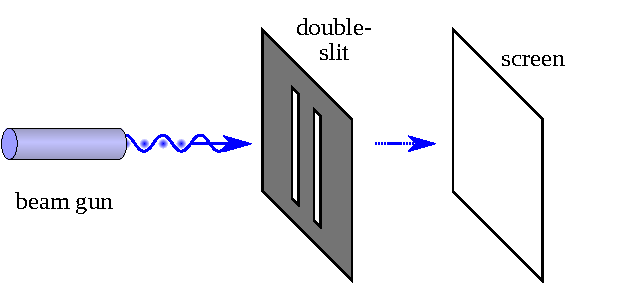
\includegraphics[width=0.6\textwidth]{light-particle-wave/Double-slit-setup.pdf}
	\caption{Experimental setup. Note that the light emitted from the beam gun (or laser) is broad enough to go through both slits.}\label{lpw:fig:2slit-setup}
\end{figure}

\begin{steps}
	\item Determine what each hypothesis \ref{lpw:hyp:part} and \ref{lpw:hyp:wave} predicts the screen will look like. Where are the dark and bright regions?
	
	\item Ask your TA for the experimental result that was done using a red laser.
	
	\item Compare the experimental outcome to the predictions and determine which, if any, of the predictions agree with the outcome, and to what degree.
\end{steps}



%Consider two lamps that are close to each other, of a single 

\subsection{Conclusion}

\begin{steps}
	\item Given the results from Situations 1 and 2 above, what judgment can you make about the hypotheses?
\end{steps}

\section{Group dynamics}

\begin{steps}
	\item Write a 100--200 word reflection on group dynamics and feedback on the lab manual. Address the following topics: who did what in the lab, how did you work together, what successes and challenges in group functioning did you have, and what would you keep and change about the lab write-up?
	
	\item Write a paragraph reporting back from each of the four roles: facilitator, scribe, technician, skeptic. Where did you see each function happening during this lab, and where did you see gaps?
\end{steps}

\section{Report checklist and grading}

The lab grade consists of 3 points for each of seven scientific ability rubric rows (the 5 listed above, which apply just to that section, as well as F1 and F2, applied to the entire report), and 9 points for providing evidence in the lab report of completing all steps of the lab, including answering every question, for a total of 30 points.
%\chapter{Observing Falling Filters}

	\begin{quotation}
		\textit{The ability to observe without evaluating is the highest form of intelligence.} \sourceatright{Jiddu Krishnamurti}
	\end{quotation}

While Mr.\ Krishnamuri may be making a stretch with his superlative, it remains true that observing without evaluating is essential for the creation of knowledge.
In our lives, we have bias (conceptions, self-constructed mental models) that we use as our lens to view the world.
These models are based on how each of us were socialized and on our subsequent experience.
To learn and create new knowledge, we must develop skill in observation.
In this lab, we will direct you to make detailed, careful quantitative observations, describe the patterns you find with mathematics, and finally make some wild guesses (``hypotheses'') about a more universal principle that explains this pattern that one could use to make predictions.
Due to time and brain constraints, we will not, in this lab, test those hypotheses.

\section*{Learning Goals}

 \begin{itemize}

  \item Conduct an observation experiment, including collecting data, finding and describing a pattern quantitatively, including presentation of data graphically and formulating a quantitative hypothesis.

  \item Use measurement uncertainty to describe physical quantities meaningfully.
  
  \item Format a lab report in a helpful way.
 \end{itemize}

\section*{The Scientific Cycle\protect\footnote{adapted from \cite{etkina_college_2014}}}

Astrophysics is an experimental science. To answer questions, astrophysicists do not just think and dream in their offices but constantly engage in experimental investigations. Astrophysicists use special measuring devices to observe phenomena (natural and planned), describe their observations (carefully record them using words, numbers, graphs, etc.), find repeating features called patterns (for example, the distance traveled by a falling object is directly proportional to the square of the time of flight), and then try to explain these patterns. By doing this, astrophysicists describe and answer the questions of ``why'' or ``how'' the phenomena happened and then deduce quantitative rules called mathematical models that explain the phenomena.

However, a deduced explanation or a mathematical model is not automatically accepted as true. Every model needs to undergo careful testing. When astrophysicists test a model, they use the model to predict the outcomes of new experiments. As long as there is no experiment whose outcome is inconsistent with predictions made using the model, it is not disproved. However, a new experiment could be devised tomorrow whose outcome is not consistent with the prediction made using the model. The point is that there is no way to ``prove'' a model once and for all. At best, the model just hasn't been disproven yet.

A simple example will help you understand some processes that physicists follow when they study the world. One model for the scientific process will also be described (there are other helpful models, and there is no one true ``scientific method''). Imagine that you walk into the house of your acquaintance Bob and see 10 tennis rackets of different quality and sizes. This is an \textbf{observational experiment}. During an observational experiment, a scientist collects data that seem important. Sometimes it is an accidental or unplanned experiment. The scientist has no prior expectation of the outcome. In this case, the number of tennis rackets and their quality and sizes represent the data. Having so many tennis rackets seems unusual to you, so you try to explain the data you collected (or, in other words, to explain why Bob has so many rackets) by devising several hypotheses. A \textbf{hypothesis} is an explanation that usually is based on some mechanism that is behind what is going on, or it can be a mathematical model describing the phenomenon. One hypothesis is that Bob has lots of children and they all play tennis. A second hypothesis is that Bob makes his living by fixing tennis rackets. A third hypothesis is that he is a thief who steals tennis rackets.

How do you decide which hypothesis is correct? You may reason: if Bob has many children who play tennis, and I walk around the house checking the sizes of clothes that I find, then I will find clothes of different sizes. Checking the clothing sizes is a new experiment, called a \textbf{testing experiment}. A testing experiment is different from an observational experiment. In a testing experiment, a specific hypothesis is being ``put on trial.'' This hypothesis is used to construct a clear expectation of the outcome of the experiment. This clear expectation (based on the hypothesis being tested) is called a \textbf{prediction}. So you conduct the testing experiment by walking around the house checking the closets. You do find clothes of different sizes. This is the \textbf{outcome} of your testing experiment. Does it mean for absolute certain that Bob has the rackets because all of his children play tennis? No; he could still be a racket repairman or a thief. Therefore, if the outcome of the testing experiment matches the prediction based on your hypothesis, you cannot say that you proved the hypothesis. All you can say is that you failed to disprove it. However, if you walk around the house and do not find any children's clothes, you can say with more confidence that the number of rackets in the house is not due to Bob having lots of children who play tennis. Still, this conclusion would only be valid if you made an \textbf{assumption}: Bob's children live in the house and wear clothes of different sizes. Generally, in order to reject a hypothesis, you need to check the additional assumptions you made and determine if they are reasonable.

Imagine you have rejected the first hypothesis (you didn't find any children's clothes). Next, you wish to test the hypothesis that Bob is a thief. This is your reasoning: \textit{If} Bob is a thief (the hypothesis), \textit{and} I walk around the house checking every drawer (the testing experiment), \textit{then} I will not find any receipts for the tennis rackets (the prediction). You perform the experiment and you find no receipts. Does it mean that Bob is a thief? He might just be a disorganized father of many children or a busy repairperson. However, if you find all the receipts, you can say with more confidence that he is not a thief (but he could still be a repairperson). Thus it is possible to disprove (rule out) a hypothesis, but it is not possible to prove it once and for all. The process that you went through to create and test your hypothesis is depicted in Figure~\ref{me:fig:isle}. At the end of your investigation you might be left with a hypothesis that you failed to disprove. As an astrophysicist you would now have some confidence in this hypothesis and start using it for practical applications, or \textbf{application experiments}.

\begin{figure}
	\centering
	\includegraphics[width=0.7\textwidth]{measurement/islegraphic.png}
	\caption{A model of the process some scientists go through to create knowledge.\cite{etkina_millikan_2015}}\label{me:fig:isle}
\end{figure}

\section*{Observation experiment: Observing falling filters}

In today's lab, you will investigate the relationship between the size of coffee filters and how long it takes them to fall. In the first section, you will determine the size of the coffee filters. In the second, you will determine how long each take to fall, controlling for other variables, and then find a mathematical pattern that describes the relationship. Note that this lab does not include any hypothesis testing.

\begin{framed}
	\textbf{Self-assessment:} To help you improve your scientific abilities, we provide you with self-assessment rubrics.
	A rubric is a scoring system.
	Self-assessment is determining how well you performed a particular task.
	So, these self-assessment rubrics are designed to help you evaluate your performance while you are designing and performing your experiment.
	
	The complete set of rubrics is available in Appendix~\ref{cha:rubrics}.
	In each lab, your report will be assessed using Rubric F, found in Table~\ref{rubric:f}, as well as 5 additional rubric rows listed in that lab.
	Each week, read through these and use them to evaluate your work as you design and perform the experiment.
	Your instructor will use the same rubrics to determine part of your grade for the lab.
	We will use the other rubrics in future labs.
\end{framed}	

\textbf{Rubrics to focus on during this experiment:} B5, B7, B8, F1, F2, G1, G2. See Appendix~\ref{cha:rubrics} for details.

\textbf{Available equipment:} several differently-sized coffee filters, meter stick, balance or scale, stopwatch, scratch paper%, camera (on your phone), Computer with ImageJ installed, string

\subsection{How big are the filters?}

% DevNote: I decided to not make this a whole application experiment with 2 different methods, for the sake of time. I also removed image analysis with ImageJ, for the same reason. --bbarker, 2018-10-02

\textbf{Goal:} Find the cross-sectional area of each coffee filter and make a determination of that area, including uncertainty in that area, for use in the next section.
%In Stage 1 of the Barker X-Prize, each team has been tasked with determining precisely how big various objects are, including marbles, cotton balls, and coffee filters, including a detailed determination of their uncertainty of these measurements.
 
%\begin{framed}
%	ImageJ is an image analysis program that includes, among other things, the ability to measure lengths, angles, and areas in images, provided that you give it a scale for how long some reference object is in the image.
%\end{framed}

\begin{enumerate}
	\item You may want to \textbf{decide on roles} for each group member. Example roles include Facilitator (ensures time and group focus are efficiently used), Scribe (ensures work is recorded), Technician (oversees apparatus assembly, usage), Skeptic (ensures group is questioning itself). Note that each role is responsible for ensuring that the thing happens, rather than necessarily doing it themselves. 
	
	\item Review Rubric G (Table~\ref{rubric:g}) and discuss any unclear expectations with your group and the instructor.
	
	\item Discuss with your group what cross-sectional area means and why it might affect the fall time. Feel free to use your resources (books, internet, etc.) to do this.
	
	\item Brainstorm different methods you could use to determine the cross-sectional area. Feel free to play with the equipment as desired. Here are some things to consider:
	\begin{itemize}
		\item Will you measure the area directly, or will you measure something else and use that to calculate the area?
		
		\item With any method, you will probably make one or more assumptions about the shape of the filter. How valid are those assumptions?
		
		\item For each method you consider, there may be different sources of uncertainty --- the resolution of the measuring devices themselves, how you use them to measure, etc. If there is a source of random uncertainty, then you will need to take several measurements and use Appendix~\ref{unc:random} to determine the uncertainty. The decision of how many measurements to take is a trade-off between increasing precision (decreasing the uncertainty of the mean) and decreasing the time the measurement process takes.
		
		\item If you make a measurement and use that measurement in an equation to find the area, you will need to propagate uncertainty as described in Appendix~\ref{unc:sec:prop}.
	\end{itemize}
	% Come up with two independent methods for determining the cross-sectional area. The purpose is that if you make a mistake or wrong assumption in one method, then the method (hopefully) gives a different result than the other method. For discovering new things, this is one quantitative way of checking your work, since you don't have the answer ahead of time.
	
	
	
	\item Decide on your method and discuss it with an instructor before you begin. They will help increase the chances that your method will lead to successful results, or at least that the unhelpful path that you choose will take a short enough amount of time for you to change it when you discover it does not work. We want you to have productive failure that you have time to learn from.
	
	\item Write down an outline of your intended procedure. You might end up changing this as you go, but it is helpful to start with a plan and then change it, rather than having no plan at all.
	
	\item For your procedure, list the sources of uncertainty involved with each measurement. For each source, identify whether it is a random or instrumental uncertainty.
	
	\item Execute your procedure, including setup, data collection, calculation of area, uncertainty estimation and propagation.
	
	\begin{framed}
	At the end of this step, you should have a table of coffee filter cross-sectional areas, with uncertainties.
	\end{framed}
	
	\item Once you are done collecting this data, review your written procedure and correct it to match what you actually did, and ensure you have sketched any measurement setups, so you can include it in the lab report. In particular, ensure that you have enough written so you can demonstrate Rubric Rows F1, G1 and G2 in your report (see Tables~\ref{rubric:f} and \ref{rubric:g}).
	
\end{enumerate}
 
\subsection{How fast do the filters fall?}

\textbf{Goal:} Determine how long it takes each coffee filter to fall.

\begin{enumerate}
	\item Review Rubric B (Table~\ref{rubric:b}) and discuss any unclear expectations with your group and the instructor.
	
	\item Identify any variables (things that could change between measurements --- either between measurements of the same filter, or among different filters) that could affect the fall time other than the coffee filter's cross-sectional area. If there is controversy in the group, feel free to test what variables might affect that fall time.
	
	\item Since you are testing how the fall time is related to the filter's area, you should hold the other variables constant, so that they affect all the filters in the same way. For each variable identified in the previous step, decide how to keep that constant.
	
	\item Brainstorm different methods you could use to determine the time it takes for the filter to fall. Feel free to play with the equipment as desired. Here are some things to consider:
	\begin{itemize}
		
		\item Will you measure the fall time directly, or will you measure something else and use that to calculate the area?
		
		\item For each method you consider, there may be different sources of uncertainty --- the resolution of the measuring devices themselves, how you use them to measure, etc. If there is a source of random uncertainty, then you will need to take several measurements and use Appendix~\ref{unc:random} to determine the uncertainty.
		
		\item If you make a measurement and use that measurement in an equation to find the time, you will need to propagate uncertainty as described in Appendix~\ref{unc:sec:prop}.
	\end{itemize}
		
	\item Decide on your method and discuss it with an instructor before you begin. They will help increase the chances that your method will lead to successful results, or at least that the unhelpful path that you choose will take a short enough amount of time for you to change it when you discover it does not work. We want you to have productive failure that you have time to learn from.
	
	\item Write down an outline of your intended procedure. You might end up changing this as you go, but it is helpful to start with a plan and then change it, rather than having no plan at all.
	
	\item For your procedure, list the sources of uncertainty involved with each measurement. For each source, identify whether it is a random or instrumental uncertainty.
	
	\item Execute your procedure, including setup, data collection, calculation of area, uncertainty estimation and propagation.
	
	\begin{framed}
	At the end of this step, you should have a table of coffee filter cross-sectional areas, with uncertainties, with another column for fall time, with uncertainty in the fall time.
	\end{framed}
	
	\item Once you are done collecting this data, review your written procedure and correct it to match what you actually did, and ensure you have sketched any measurement setups, so you can include it in the lab report. In particular, ensure that you have enough written so you can demonstrate Rubric Rows B5, F1, G1 and G2 in your report (see Tables~\ref{rubric:b}, \ref{rubric:f}, and \ref{rubric:g}).
\end{enumerate}

Now that you have these measurements, it is time to find a pattern.

\subsection{Finding a pattern}

The penultimate step in an observational experiment is to find a pattern. Note that we are not explaining why this pattern is happening yet --- we are focusing on describing it first.

\textbf{Goal:} Find a pattern in the data and describe it mathematically.
\textbf{Available equipment:} Computer with spreadsheet software

\begin{enumerate}
	\item Use a plotting program, for example LibreOffice Calc or Microsoft Excel, to plot a graph of fall time vs. filter area. The independent variable should be on the horizontal axis. The axes should each be labeled with the quantity name and the unit in parentheses. For example, if you measured fall time in seconds, then the axis label should be something like ``fall time (s)''.
	
	\item In that graph, include also the uncertainty in each value. This usually involves right-clicking on a data point and selecting ``error bars''. Then you can highlight the column of cells that include the uncertainties.
	
	\item Visually, discuss what shape the data points make. Speculate what kind of relationship you see. Is it proportional? Linear? Parabolic? Exponential? Logarithmic?
	
	\item Create a line of best fit (or ``trend line'') in the graph using the software. Choose the equation type to match what your group guessed in the previous step. If the line obviously does not match the data, try again with a different equation type. Quantitatively, the goodness of fit of a line (how close the line is to your data points) can be represented by the correlation coefficient, given as $r^2$ in the software. If $r^2 \gtrsim 0.8$, then the equation that you found describes the data fairly well.
	
	\item Review Rubric Rows B7 and B8 in Table~\ref{rubric:b} and ensure that you are demonstrating them here or have enough information to do so in your lab report.
\end{enumerate}

\subsection{Finishing up}

XXXX TO FINISH XXXX

what to include in lab report

extra fun: extrapolate to 0 area, compare with freefall time.

%Rationale:
%\begin{enumerate}
% \item want one experiment where students measure lengths and estimate uncertainties that are needed for data analysis. Lengths are intuitive things for students, no prior teaching needed. Then they see how those lengths compare to something else in a physics-y way. Then they graph it and decide what functions might describe them.
 
% \item falling and air resistance is good here. air resistance depends on cross sectional area, so length measurement. Data is not simple and obvious, but is instead messy, making pattern identification non-trivial, but still possible. Also cannot just use or look-up simple answers online -> authentic inquiry.
 
% \item so could do area vs. time to hit the floor. Can measure with video tracking, photogates, motion detector, stopwatch. need multiple sizes of coffee filters.
 
% \item Or position vs. time for different objects. This should give some interesting graphs, since objects can vary from no-meaningful-air-resistance to dominated-by-air-resistance constant. And the latter case should have an acceleration at the beginning, then constant, so it's more complicated. Must use video tracking or motion detection. So includes the skill of choosing with data to model. is there one function that works for all parts, or is there a transition between different situations?
 
% \item for video tracking, need to know how students can find framerate of videos they take, make sure it's easily imported to OSP Tracker.
%\end{enumerate}

\section{If in Stars class, also do this:}
\subsection{Remote Observing with the Stone Edge Observatory}

For two labs in this course, we will be taking observations remotely with the Stone Edge Observatory in Sonoma, California. We will use a queuing system to submit observations that are automatically scheduled and taken by the telescope. The data are then processed and typically available for analysis several days after they were obtained. To ensure that our data are taken and reduced in time for our in-lab analysis (which is subject to possible delays due to, e.g., the weather at the observing site), we will be submitting observations to the queue several weeks prior to lab in which they will be analyzed.

First, you will need to register for an account that will allow you to access the queue website. Make groups of two to three students so that there are no more than 5 groups in a section. Each group will use one member’s email to sign up for an account in the queuing system. A TA will be present to manually add each group. Each group will receive an email that will allow them to create an account. Since you will be sharing an account, be sure to share the account password (and obviously don't re-use one from another personal account).

Once you have an account, you will be able to log onto the queue and submit observations. To do so, go to the website \texttt{https://queue.stoneedgeobservatory.com/} and log-in with your group's credentials. Then navigate to \texttt{OBSERVATIONS} $\blacktriangleright$ \texttt{SUBMIT AN OBSERVATION}. This will take you to a form that allows you to input the specifics of your observation. These will be given to you for each lab.

\subsection{HR Diagram: Taking observations}
For this lab, each section will be taking observations of one of two star clusters --- NGC 869 and M15. You will then use this data to make color-magnitude diagrams of these clusters, which can then be compared with stellar evolution models to determine when these clusters formed. Table~\ref{hr_diagram_obs} lists the parameters for the observations to be taken in this lab - each section will be assigned a cluster, and each group in the section should submit one observation. Each group will then analyze their data in-lab, and will combine datasets. If there are fewer groups than observations, omit the longest-exposure observations.

\begin{table}
    \centering
    \caption{HR Diagram Lab Observations}
    \label{hr_diagram_obs}
    \begin{tabular}{|l|c|c|c|c|r|}
    \hline
    \textbf{Program} & \textbf{Target} & \textbf{Exp Time (s)} & \textbf{Exp Count} & \textbf{Bin}
         & \textbf{Filters} \\
    \hline
    General & M 15 & 1 & 1 & 2 & Dark, g', r'\\
    \hline
    '' & '' & 5 & '' & '' & '' \\
    \hline
    '' & '' & 10 & '' & '' & '' \\
    \hline
    '' & '' & 20 & '' & '' & '' \\
    \hline
    '' & '' & 40 & '' & '' & '' \\
    \hline
    '' & NGC 869 & 0.5 & '' & '' & ''\\
    \hline
    '' & '' & 1 & '' & '' & '' \\
    \hline
    '' & '' & 2 & '' & '' & '' \\
    \hline
    '' & '' & 5 & '' & '' & '' \\
    \hline
    '' & '' & 10 & '' & '' & '' \\
    \hline
    \end{tabular}
\end{table}

\section{Post-lab survey}

[Include Anna Karelina's flow questions here]

%\chapter{Radioactivity Part 1}

\section{Introduction}

Over the next two weeks, we will explore a few basic properties of radioactive decay: (1) counting statistics, (2) types of radioactive decay, and (3) half-life. In the first week, we'll use samples of radioactive materials --- isotopes of cobalt, strontium, cesium, and polonium --- to generate energetic particles. We'll then make measurements to explore the properties of these particles and the counting statistics related to their decays. In the second week, we’ll produce our own short-lived isotope of silver and watch the new atoms decay by counting the number of particles they emit. From that, we will measure the so-called half-life of the silver isotope we produce.

\subsection{Learning Goals}

\begin{itemize}
	\item Become familiar with the statistics of counting events.
	
	\item Describe the four types of radioactive decay products
	
	\item Identify sources of random and systematic error.
	
	\item Make careful measurements.
	
	\item Use a spreadsheet application to calculate and plot data.
	
	\item Relate small scale physics (studying atoms in the lab) to large scale astrophysics (dating the big bang, supernovae, and the solar system)
\end{itemize}

\subsection{Scientific Background}

Nuclear reactions play an important role in astronomy, geophysical sciences, archaeology, and physical anthropology. They explain energy generation in stars, the relative abundance of chemical elements, and provide a method for determining the age of things --- from a piece of wood, to a meteorite, to the universe itself.

Most elements exist in a number of different forms, called isotopes, some of which are unstable and can change from one type of element to another. When this occurs, a high-energy particle is usually emitted from the nucleus of the element as it changes. By measuring the ratios of isotopes with differing decay rates, one can infer the age of an object.

\section{Testing experiment: Do radioactive isotopes decay randomly?}

\textbf{Goal:} Answer the question, ``Given what we understand about the standard deviation of measurements of random processes, do radioactive isotopes decay randomly?'' Or, in the frame of a testing experiment, test the following hypothesis: ``Radioactive sources decay randomly.''

\textbf{Available equipment:} Stopwatch, SpecTech Geiger counter, computer with spreadsheet software, radioactive source ($^{137}$Cs)

\begin{framed}
	\textbf{Warning: Radioactive Material!} The radiation levels are very low and they present no hazard for the short time that you are in the lab. We estimate that you will receive an additional $10\:\mu$Sv dose of ionizing radiation for the time that you are in lab today, about the same as you receive every day normally. You can compare this to the example doses in Fig.~\ref{rad1:doses}. Here are tips to keep your exposure low:
	\begin{itemize}
		\item \textbf{Do not have any food, drink, food containers, or make-up on the lab bench, and do not consume any food or drink, and do not apply make-up, in the lab.} These might get irradiated and become radioactive themselves, and when you eat them, you might get dose internally, where your skin is not present to protect you.
		
		\item \textbf{Decrease time with and increase distance from sources.} Handle the sources only when you need to be for the lab, and return them to their container when not using them.
	\end{itemize}
\end{framed}

\begin{framed}
	\textbf{Caution: Fragile Equipment!} The Geiger tube (the upright cylinder sitting in the plastic stand and connected to a coaxial cable at the top) hold a gas under vacuum, with a thin, fragile window at the bottom of the tube. Do not touch it, as it breaks extremely easily.
\end{framed}

\begin{figure}
	\centering
	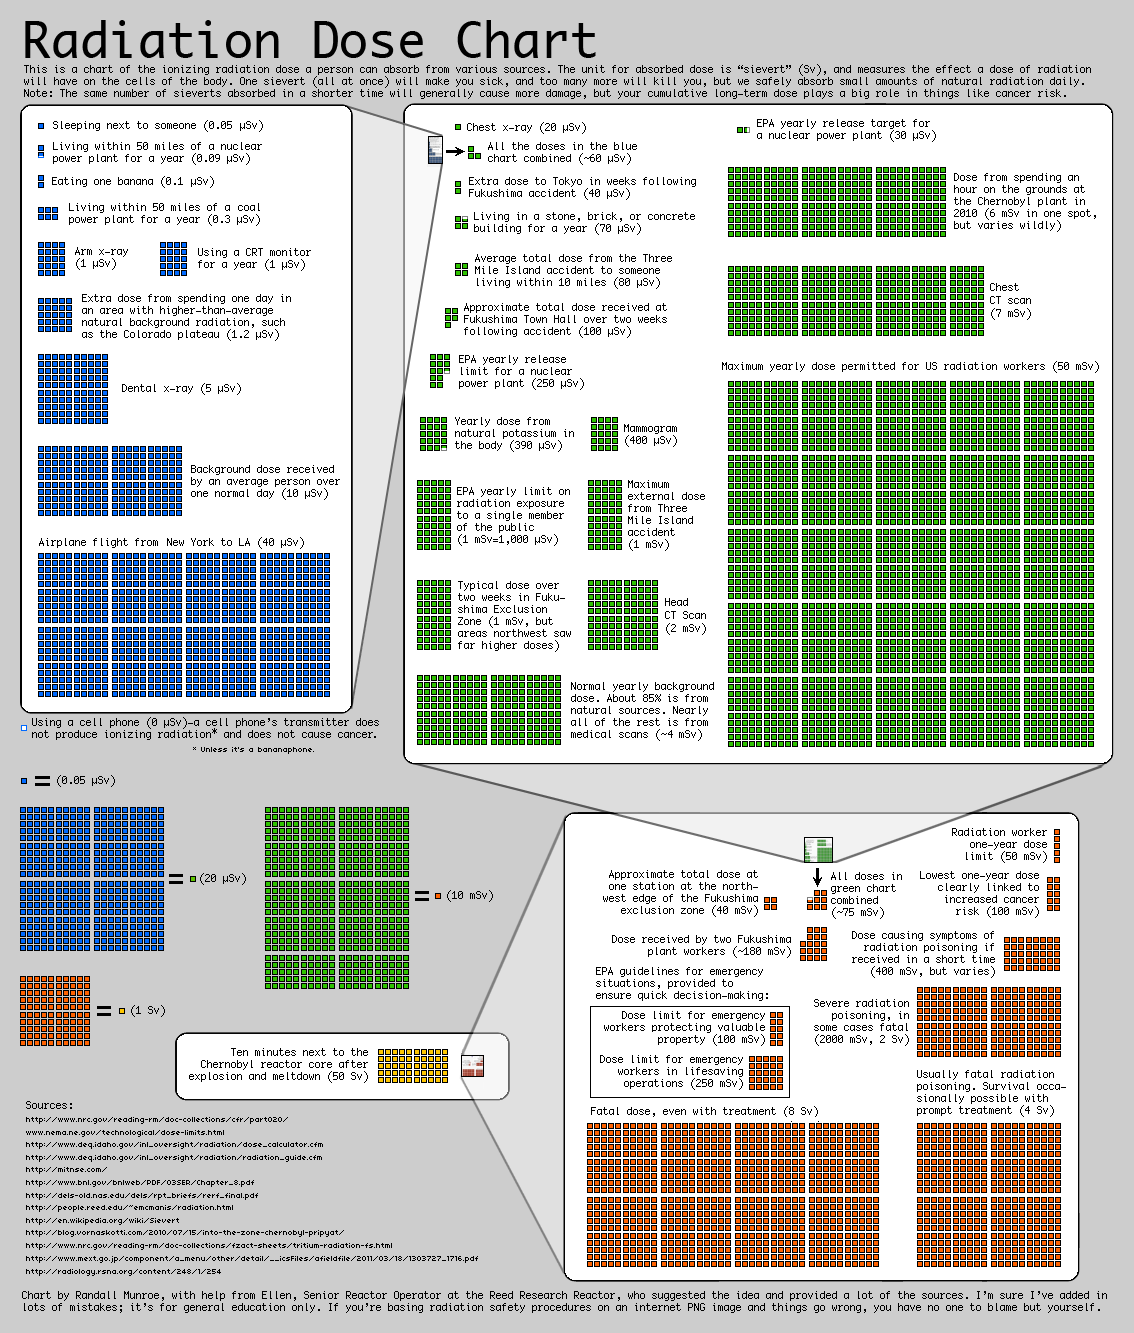
\includegraphics[width=\textwidth]{radioactivity-1/radiation-xkcd}
	\caption{A chart of ionizing radiation dose from various sources. Source: \url{https://xkcd.com/radiation/}}\label{rad1:doses}
\end{figure}

\textbf{Rubrics to focus on during this experiment:} C1, C4, C7, C8, F1, F2, G2. See Appendix~\ref{cha:rubrics} for details.

\subsection{Theory of counting statistics}

If you've ever worked in a not-too-busy retail environment, you’ve probably had the
experience of realizing (perhaps) that random and uniform are two quite different things.
You no doubt have sat waiting for customers, with nobody around for long stretches of
time, and then, as though they'd coordinated in advance, a half dozen people all show up
within a few minutes of each other. Each customer is indeed independent (no, they didn't
have a Twitter call to organize a flashmob!\footnote{Yes, popular interest in flash mobs peaked in 2011. Bear with us here.}) yet their arrival times clearly appear clustered. They are, in fact. But randomly. Uniform – one customer each minute – is quite dramatically different than a random procedure that yields one customer per minute on average. Retail customers (to a great extent), and elementary particles, act randomly, not uniformly.

Each atom in a radioactive sample has, per unit time, some probability of undergoing
radioactive decay. That probability is independent of all the other atoms in the sample.
Each atom decays, or not, based on its own probability and no other. The ensemble of
particle decay counts that one would measure in the sample (using a Geiger counter as we will
do, for example) is described by the something called the Poisson distribution, which
gives, in this instance, the probability of a integer number of events occurring in a fixed
interval of time, given an average rate. For large count rates, like we have here, the
Poisson distribution is indistinguishable from the normal distribution (that is, a simple
Gaussian function).

Specifically, for a process that produces an average $\bar{N}$ counts in a certain time duration (in the case of large $N$), the expected measurement of that count for that time duration is a
random draw from a normal distribution with mean $\bar{N}$ and a standard deviation of
$\sqrt{N}$.

\subsection{Doing the experiment}

\begin{enumerate}
	\item To find the steps of a testing experiment, review Rubric C, found in Table~\ref{rubric:c}.
	
	\item\label{rad1:step:predict-random} A prediction is what the hypothesis says will happen in the event of a particular experimental procedure. Given the hypothesis stated in the goal, and the theory described above, if you collect a series of counts of radioactive decay, what does the hypothesis predict the standard deviation of those counts should be equal to? Record this prediction in your lab notebook.
	
	\item \textbf{Collecting data.} In order to find the standard deviation of a number of measurements, you will need to take those measurements. In the following steps, you will do 10 trials of measuring the count rate (counts per unit time) during periods of about 30 seconds, then take the standard deviation of those 10 trials. Since you will not be able to stop the counter after exactly 30 seconds, you will divide the displayed count by the displayed time to get a count rate (in units of ``counts per second'').
	
	\begin{framed}
		\textbf{The Apparatus.}
		
		For this lab and the following one, you will be provided with a number of different radioactive materials packaged in small plastic disks. Note that each disk has the name of
		the isotope (e.g.\ $^{60}$Co), the type of radiation, and the half-life printed on one side of the
		sample. Half lives can range from fractions of a second to billions of years, depending on
		the isotope.
		
		The energetic particles produced in radioactive decay reactions can be detected by a
		device called a Geiger counter. This consists of a tube filled with inert gas with a wire
		running through it. A high voltage is applied between the wire and the tube. When a high-
		energy particle enters the tube, it can ionize the gas. The freed electrons produce a brief
		pulse of current at the output of the device. The pulses can then be counted.
		
		The counter itself is controlled using buttons on the front panel. \texttt{COUNT} begins the count
		and starts the timer, \texttt{STOP} pauses the count and timer, and \texttt{RESET} sets the count and
		timer to zero. Use the dial on the counter to change the display between the count and the
		elapsed time. When you first turn on the Geiger counter you need to set the voltage to
		$1000\:$V --- the TA will demonstrate how. \textbf{Caution:} Do not turn off the voltage during the
		experiment; use the \texttt{STOP} button to stop the count. \textbf{Do not touch the window on the
		bottom of the tube, as it breaks extremely easily.}
	\end{framed}
	\begin{enumerate}
		\item Take one of the $^{137}$Cs disks and place it printed side down in the plastic shelf shaped to hold it, and place that shelf in the slot second from the top in the stand under the Geiger counter. Note that if you have the Geiger counter on, that it is measuring a large count rate.
		
		\item Use the controls \texttt{COUNT}, \texttt{STOP}, and \texttt{RESET} to measure the number of counts in 10 approximately 30-second intervals. Use the dial on the display to access both the counts and the elapsed time. The provided stopwatch may also help you organize your effort --- \textit{but use the time from the Geiger counter apparatus directly} for your calculations.
		
		\item Record the counts and elapsed time in each interval in a spreadsheet and calculate the count rate in counts per minute (``cpm'' for short).
	\end{enumerate}

	\item \textbf{Analysis.} Note that the count rate is not identical in each trial, even though you accounted for the different measurement durations. Let's see how far away the standard deviation here is from the prediction in Step\ref{rad1:step:predict-random}. Calculate the standard deviation of these measurements. How close is it?
	
	\item Qualitatively, it might appear close or far away, but to test the hypothesis, you should take into account the uncertainty of the standard deviation. This is, effectively, the \textit{standard deviation of the standard deviation}. You would need to take, for example, 10 trials of these 10 trials and compute the standard deviation of that. Fortunately, you have other lab groups who are doing the same experiment. Share the standard deviation you found with the other lab groups, calculate the average and standard deviation of those standard deviations, and use Appendix~\ref{unc:sec:comparing} to compare your average standard deviation to the prediction that your hypothesis made.
	
	\item Use this quantitative comparison to determine if the prediction and the outcome agree or not.
	
	\item Based on that agreement, and taking into account the experimental conditions, make a judgment about the hypothesis.
\end{enumerate}
%\chapter{Radioactive Half-Life}

%TODO add instructor note: to close door to KPTC 003, need to toggle switch that keeps it open, which is above the door.

%TODO add notes about neutron howitzer from https://wiki.uchicago.edu/display/phylabs/Mass+of+the+Neutron and from this email from David McCowan:
%The source is a mixture of plutonium and beryllium. The plutonium decays via alpha emission and the beryllium absorbs the alpha to become carbon + a free neutron. The neutron has an energy given by a very complicated distribution, but the energy distribution goes up to ~11 MeV. The paraffin shielding (and the lucite in the plug) slows down neutrons, so that anything which escapes is thermalized such that E ~ kT ~ 1/40 eV. At the point where the foils are placed, the neutrons have been slowed some, but not completely... if they are a full 11 MeV still, they are too energetic to bind with the silver, so the foils are absorbing from the lower end of the spectrum or from neutrons that have scattered enough material to have less energy than they started with.
%
%The activity of the Pu-Be core is an astounding 5 Ci (!!), but that's the alpha flux which doesn't penetrate out of the core. The neutron flux is considerably less. Looking back at the original purchase order, it looks like we have 80 g of plutoinium mixed with 41 g of beryllium and a listed (I think unshielded?) emission rate of 9 x 10^6 N/sec.

%TODO include suggestion to video the counter and a stopwatch to get more accurate 30-sec readings.

Building on our work from last week, we will continue to study the radioactive decay.
The physical laws of radioactivity predict that the rate of decay (number of atoms
decayed / time interval) is proportional to the number of radioactive nuclei present. This
is due, as we saw in counting statistics previously, to the independence of the decay of
each atom in the sample. The proportionality constant that describes the decay rate
depends on the specific radioactive nucleus. A concise and suggestive way to
characterize the nucleus is by its half-life, the time it takes for the number of radioactive
nuclei to decrease to half of the initial value. You will obtain data to check the form of
the law and to determine the half-life of one or more isotopes of silver.

We will use a device known as a neutron ``Howitzer''. It consists of a source of alpha
particles and a material that absorbs alpha particles and immediately decays by emitting
neutrons. (The neutrons shoot out from the barrel of the shielded volume, vaguely like
shells from WWI artillery, hence the name.)

\section{Background}

We will let the neutrons bombard a small sample of the stable isotope of silver, $^{107}$Ag, to
produce $^{108}$Ag, via the reaction
\begin{equation}
 ^{107}\textrm{Ag} + \mathrm{n} \rightarrow\, ^{108}\textrm{Ag} + \gamma \,,
\end{equation}
where $\mathrm{n}$ represents a neutron and $\gamma$ a gamma particle --- that is, a high energy photon.

The radioactive isotope of silver, $^{108}$Ag, spontaneously decays to an isotope of cadmium
with the same mass number, $^{108}$Cd, by the reaction
\begin{equation}
 ^{108}\textrm{Ag} \rightarrow\, ^{108}\textrm{Cd} + \mathrm{e}^- + \gamma \,,
\end{equation}
where $\mathrm{e}^-$ is an electron (that is, a $\beta$ particle, as we saw and measured last week).

Your TA will bombard silver foils with neutrons using the neutron howitzer. Some of the
nuclei in the foil will have captured a neutron and transformed into a different isotope
which is unstable and can be detected via their decay products. Each group will be given
one of these silver foils.

\section{Procedure}

\textbf{Rubric rows to be assessed:} D1, D4, F1, F2, G2, G3 (ignore actually doing it), G4

Your task is to measure the half-life of $^{108}$Ag. We will use the Geiger tube to count
decays. That is, we will count the $\beta$ particles --- the gamma rays make only a small
contribution to the counts in this instance. You should attempt to carry out the counting
fairly quickly after the silver foil is removed from the howitzer as the decay time is quite
short.

Before the neutron irradiation begins you will want to record the background rate. Press
\texttt{STOP} and \texttt{RESET} on the counter to set the display to zero. Next, press \texttt{COUNT} with no
sample below the Geiger tube and collect the total number of background counts, $N_\textrm{bkg}$ ,
that accumulate in approximately 5 minutes. Once 5 minutes has elapsed press \texttt{STOP} to
end the count. Turn the dial to \texttt{TIME} and record a precise measurement of the elapsed
time, $t$, in seconds. The background rate $R_\textrm{bkg}$ is found with
\begin{equation}
R_\textrm{bkg} = N_\textrm{bkg} /t
\end{equation}
with an uncertainty given by Poisson statistics. Report both the background rate and uncertainty in your lab report.

While the samples are being irradiated, set up your measurement apparatus. Once the samples are ready, quickly place a silver foil sample in the tray below the Geiger tube. Using a stopwatch and the
counter, record the number of counts and the time at 30 second intervals for
about 10 minutes, continuously. Unlike last week's lab with the same apparatus, you will
be recording data continuously, and so will need to use the watch to record times rather
than timer built into the Geiger counter. Record your data.

\section{Calculations}

The experimental data will be used to determine a half-life (or half-lives). We know that
the decay rate ($R=\Delta N / \Delta t$) of a radioactive nuclide is proportional to the number of nuclei present. The proportionality constant is called the decay constant $\lambda$, and the equation that describes what was just discussed is
\begin{equation}
 R = \lambda N \,,
\end{equation}
where $N$ is the background-subtracted counts. Using integral calculus and the above equation, we find
\begin{equation}
 N = N_0 e^{-\lambda t} \,,
\end{equation}
where $N_0$ is the number of nuclei at the initial time $t=0$. The half life $T_{1/2}$ is defined by
the time it takes for $N = N_0 /2$ and is related to the decay constant by $T_{1/2} = \ln(2)/ \lambda$, where
$\ln()$ is the natural logarithm function, and so $\ln(2) \approx 0.693$.

We can now write the radioactive decay equation as
\begin{equation}
 R = \lambda N_0 e^{-t \ln(2) / T_{1/2}} \,.
\end{equation}
Taking the logarithm of both sides and substituting for $N$ gives
\begin{equation}
 \ln(R) = - \left(\frac{\ln(2)}{T_{1/2}} \right) t + \mathrm{const} \,.
\end{equation}
Your TA will help you to understand the details of this derivation.

Make a plot showing $\ln(R)$ on the vertical axis and elapsed time, $t$, along the horizontal
axis. Don’t forget to subtract the background where appropriate. Calculate the slope
and use this value to solve for the half life using the above equations. Report this value
along with a table of your decay rate data and the plot described above.

\section{Questions (these should be included in your lab report)}

\begin{enumerate}
	\item Look up the half-lives of the various nuclides of silver. What is the published
	half-life of the nuclide you’re observing? How does this compare with your
	calculated result? Calculate the percent difference in your result.
	
	\item For the silver foil, how long would it take before you would expect to detect only
	one count per second, background corrected?
	
	\item The detector only measures particles that travel up into the detector. The majority
	of particles traveling in the other directions escape detection. Will this short-
	coming affect the measured half-life? If so, how? If not, why not?
	
	\item Describe one thing you could change in this experiment that could lead to a more
	accurate measurement of the half-life of the silver isotope.
	
	\item The particular irradiated silver sample you used contained some unknown
	percentage of the unstable silver isotope, and was irradiated at some unmeasured
	time before you began your experiment. Does this matter to your results? Explain.
	
\end{enumerate}
%\chapter{Local Gravitational Field}

One of Newton's revelations was that physical laws that governed the movement of objects near Earth also predicted the movements of objects in the sky.
The apocryphal story of an apple falling on Newton's head brings to mind the mechanism of gravity --- the phenomenon of massive objects attracting each other.
In this lab, you will measure the strength that gravity has where we are, near the Earth's surface. This measurement might also enable us to learn more about the mass of the Earth itself in a future lab.

\section{Learning goals}

\begin{itemize}
	\item Understand Newton's law of universal gravitation and its linear approximation
	
	\item Identify sources of statistical and systematic error
	
	\item Demonstrate an ability to make careful measurements
	
	\item Demonstrate proficiency in basic calculations and plotting
	
	\item Explain the importance of repeated measurements and sufficiently large datasets
	
	\item Use experimentally derived quantities to obtain a mass for the Earth.
\end{itemize}

\section{Scientific Background}

\subsection{The gravitational field strength and Newton's second law}

The force of gravity, $F$, between two objects with mass $m_1$ and $m_2$ and whose centers are separated by a distance $R$ is given by Newton's law,
\begin{equation}\label{lg:eq:newtons}
 F_\textrm{gravity} = G \frac{m_1 \: m_2}{r^2} \,,
\end{equation}
where the Newtonian constant of gravitation $G = 6.67408(31) \times 10^{-11} \: \textrm{m}^3 \: \textrm{kg}^{-1} \: \textrm{s}^{-2}$. Astronomers apply Newton's law to infer fundamental information about astrophysical objects, for example the mass of binary stars. Indeed, this is one of the most common methods by which astronomers ``weigh'' astrophysical objects, including the Earth itself. For measuring the force acting on an object of mass $m$ that is affected predominantly by the Earth's gravity, the force acting on it would be
\begin{equation}\label{lg:eq:fearth}
 F_\textrm{Earth} = \frac{G M_\Earth}{(R_\Earth + h)^2} m
\end{equation}
where $M_\Earth$ and $R_\Earth$ are the mass and radius of the Earth, respectively, and $h$ is the height above the Earth.

For objects near the Earth's surface, where $h$ is much less than $R_\Earth$, $h$ can be treated as zero, resulting in a constant gravitational force, with Equation~\ref{lg:eq:fearth} reducing to
\begin{equation}\label{lg:eq:fearthred}
F_\textrm{Earth} = \frac{G M_\Earth}{(R_\Earth)^2} m \,.
\end{equation}
Notice that on the right-hand-side of this equation, the only variable is the mass. The others, together, constitute the \textit{strength of the local gravitational field}, $g$ (sometimes pronounced ``little g''). So our simplified equation is
\begin{equation}\label{lg:eq:fegm}
 F_\textrm{Earth} = g m \,,
\end{equation}
where we have made the substitution
\begin{equation}\label{lg:eq:g}
g = \dfrac{G M_\Earth}{(R_\Earth)^2} \, .
\end{equation}
Notice that we have taken a complicated inverse square equation (Equation~\ref{lg:eq:fearth}) and
converted it to a much simpler one (Equation~\ref{lg:eq:fegm}). This process is called \textit{linearization} and is a
trick astronomers often use to make calculations more manageable. You will encounter
this technique throughout this and other PHSC courses.

We see from Equation~\ref{lg:eq:g} that if we can make accurate measurements of $g$, $G$, and $R_\Earth$, we can calculate the mass of the Earth. We'll look up $R_\Earth$ online, and next week we will measure $G$. To find $g$, we note that Newton's second law of motion states that the acceleration $a$ of an object is directly proportional to the net force $F_\textrm{net}$ acting on it and inversely proportional to its mass, $m$, or, more succinctly and slightly rearranged,
\begin{equation}
 F_\textrm{net} = m a \,.
\end{equation}
If the Earth's gravity is the only force acting on our object, then $F_\textrm{net} = F_\textrm{Earth}$, and substituting Equation~\ref{lg:eq:fegm}, we find that
\begin{equation}
 g m = m a \,,
\end{equation}
and thus, simplifying,
\begin{equation}
 a = g \,.
\end{equation}
So, the acceleration of an object that is subject only to the Earth's gravity is equal to the local gravitational field strength. If we can measure the acceleration, then we can find $g$, and get one step closer to determining the mass of the Earth.

\subsection{Constantly accelerated motion}

If an object is subject to a constant force, then according to Newton's second law, it undergoes constant acceleration. If an object undergoes constant acceleration $a$, and we know the object's initial position $x_0$ and velocity $v_0$, then after a time duration $t$, we can derive using calculus that the object's position $x$ and velocity $v$ are given by
\begin{equation}\label{lg:eq:x-const-a}
 x = x_0 + v_0 t + \frac{1}{2} a t^2
\end{equation}
and
\begin{equation}
 v = v_0 + a t \,.
\end{equation}

\section{Application experiment: determine $\bm{g}$ on the Earth's surface}

\textbf{Goal:} Determine $g$ near the Earth's surface by finding the acceleration of an object undergoing freefall (no substantial forces other than gravity) using two different methods: 

\textbf{Rubrics to be assessed:} D4, D5, F1, F2, G1, G2, G4

\textbf{Available equipment:} stopwatch, dense object to drop, meter stick, camera (including the one on your phone), computer with Tracker\footnote{Open Source Physics Tracker can be downloaded from \url{https://physlets.org/tracker} and is also installed on the lab computers.} installed.

\subsection{Method 1: freefall time}

\begin{enumerate}
	\item Drop the object from a known height and measure the time to fall with a stopwatch. Do this as many times as makes sense to you.
	
	\item List the sources of uncertainty and determine whether each is a random uncertainty or an instrumental uncertainty.
	
	\item Calculate the average fall time.
	
	\item Calculate the standard deviation of the average fall time (using Equation~\ref{unc:eq:stdevmean}), and report the latter as the uncertainty in the average fall time.
	
	\item Use the average fall time and the initial position and velocity of the object to calculate the acceleration.
	
	\item Propagate the uncertainty in the time and position to find the uncertainty of your measured acceleration (see Section~\ref{unc:sec:prop})
	
	\item Report the acceleration found by this method as ``value $\pm$ uncertainty [units]''. For example, $9.73 \pm 0.04\:$m/s$^2$.
\end{enumerate}

\subsection{Method 2: Video tracking}

It is helpful to use two methods to find the same quantity, so that mistakes or incorrect assumptions made in one method do not carry over to the other, and are thus more likely to be detected. In this method, you will record a video of an object falling, make a position vs. time plot, and fit the constant acceleration equation (Equation~\ref{lg:eq:x-const-a}). You will use a computer program to make this analysis easier.

\subsubsection{Record the video}

\begin{enumerate}
	\item Find a good object to drop. It should be dense enough to not be slowed down significantly by air resistance.
	
	\item Using the camera on one of your group member's phones, record a video of the object falling.
	
	Here are some tips to get a quality video:
	\begin{itemize}
		\item Include an object of known length in the shot, at the same distance from the camera as the falling object. This gives a reference length, so that you can find how each camera pixel scales to the physical situation.
		
		\item Avoid parallax error by having the object be at about the same distance from the camera throughout the fall. Having the camera be farther away can help. Also, you can ensure that the top and the bottom of the fall are the same distance from the camera.
		
		\item Hold the camera steady.
	\end{itemize}

	\item Record that video and transfer the video to a computer that has Tracker installed.
\end{enumerate}

\subsubsection{Importing the data into Tracker}

In this part, you'll use Tracker to record the position of the object at each timestep. To do this, you'll need to tell it what direction ``down'' is in, what the scale of the image is, and when time $t=0$ is. Then you'll record the positions, find out what parameters best fit the curve that is produced, and use those to find the acceleration.

\begin{enumerate}
	\item Open Tracker on a computer. You can install it on your own computer by visiting \url{https://physlets.org/tracker}.
	
	\item In Tracker, open your video.
	
	\item \textbf{Find frame when zero time is.} Move the slider below the video to the right to advance the frames until you find the first one in which the object is falling. Record that start frame number, which is found to the left of the slider bar in red.
	
	\item \textbf{Find the last relevant frame.} Keep moving the slider to the right until you find the last frame before the object hits the floor. Record that end frame number.
	
	\item To \textbf{tell Tracker about these frames}, click the 5th icon from the left on the toolbar above the video (``Clip settings'') and enter the start frame and end frame.
	
	\item \textbf{Tell Tracker how long things are.} In astronomy applications, this is known as the ``pixel scale''. Here we can just draw a line on the frame and tell Tracker how long that line is in real life. Click the 6th icon from the left (blue, with a ``10'') and select \texttt{New} $\rightarrow$ \texttt{Calibration Stick}. Shift-click to mark each end of your known length, and type in your known length, with units in the box that appears along the stick. Use ``m'' for meters.
	
	\item \textbf{Align the coordinate system.} In the toolbar, click the 7th icon from the left (magenta crossed lines). Click and drag the coordinate system's origin (the intersection of long lines) to the location of the object in the start frame.
	
	\item \textbf{Check to see if the camera was tilted.} Advance the video to see if the object moves along an axis. If it goes off at an angle, the camera was tilted compared to the direction of motion. In this case, rotate the coordinate system to align with the motion by clicking and dragging the small line that crosses one of the axes.
	
	\item \textbf{Tell Tracker where the object is in every frame.}
	\begin{enumerate}
		\item In the toolbar, click \texttt{Create} $\rightarrow$ \texttt{Point Mass}.
		\item Ensure the slider is at the start frame.
		\item Shift-click on the object. Notice that the frame advances to the next one automatically.
		\item Continue to shift-click to mark the object's position throughout the duration.
	\end{enumerate}
\end{enumerate}

\subsubsection{Analysis}

\begin{enumerate}
	\item \textbf{Ensure the correct axis is selected for analysis.} Look at the plot to the right of the video. If there is not a smooth-ish curved line, click on the axis label ``x (m)'' and choose instead ``y (m)''.
	
	\item In the drop-down menu, select \texttt{View} $\rightarrow$ \texttt{Data Tool (Analyze...)}.
	
	\item In the window that appears, above the plot, click \texttt{Analyze} $\rightarrow$ \texttt{Curve Fits}.
	
	\item Notice that Eq.~\ref{lg:eq:x-const-a}, which describes freefall, is a quadratic equation, which means the shape is a parabola. For ``Fit Name'', choose ``Parabola'' from the drop-down menu.
	
	\item Use the Fit Equation and Parameter Values, comparing with Equation~\ref{lg:eq:x-const-a}, to find the acceleration $a$, and thus the gravitational field strength $g$.
	
	\item To get an uncertainty for this value, use the ``rms dev'' value, which describes the average deviation of the fit equation from the points, divide that by the average (mean) position, and multiply that by your value for the acceleration. You can find the mean position by selecting \texttt{Analyze} $\rightarrow$ \texttt{Statistics} and reading above the data table column.
\end{enumerate}

\subsection{Comparing the methods, final determination of $\bm{g}$}

\begin{enumerate}
	\item Compare the values of $g$ from the two methods using the $t'$ statistic as described in Appendix~\ref{unc:sec:comparing}.
	
	\item Use that comparison and your assessment of which method had fewer questionable assumptions to decide on your final answer for $g$ (including an uncertainty). How close is it to the average $g$ described, for example, on Wikipedia?
\end{enumerate}
%\chapter{Cosmic Energy Transformations}

%TODO add Heat Death of the Universe to end of this lab.
%TODO:
% - get backup LEDs and flashlights, our own solar panels
% - cart and track worked well
% - double pendulum was too complicated
% - groups with all women could not get the fire syringe to work
% - some syringes leak air and thus don't work

\section{Background: Energy Conservation}

In every closed system, energy is conserved. Mass-energy, that is. Energy is never created or destroyed. This fact has been derived as a mathematical consequence of the fact that the laws of physics do not change over time (the relation between the two is a special case of Noether's theorem, discovered by Emmy Noether, a Jewish-German mathematician described by Einstein as the most important woman in the history of mathematics). Instead of being created or destroyed, energy is transformed from one kind to another.

There are two different kinds of energy, kinetic and potential. Kinetic is energy that something has by virtue of it moving (the faster it is going, the greater the kinetic energy), and potential is stored energy that something has because of its particular position in relation to something else. It is called ``potential'' because it gives the object the potential to do something. There are many different kinds of potential energy, depending on the situation. Examples include gravitational (being further away from massive bodies), chemical (sugar, batteries), electric (electric current), electromagnetic radiation (light, infrared, x-rays), elastic (springs, rubberbands), thermal (warmth), and nuclear (isotopes that can break down or combine to release energy).

We can use the principle of energy conservation to learn about physical processes. For example, if a car is traveling (kinetic energy) and is turned off and slows down and stops, the kinetic energy decreases. That energy did not disappear --- it was either transformed into thermal energy through friction in the brake pads or road, or was stored up again as electrical energy (in the case of regenerative braking in electric vehicles). We even know how much --- the amount of kinetic energy lost is the exact amount of energy gained in these other forms.

%This principle was used to discover neutrinos. In certain radioactive decay, electrons were  particles so unheavy that they were originally thought to have zero mass, and we only know that they have different masses, but not what they are.

%\section{The cosmic Rube Goldberg machine}

\begin{steps}
	\item Since energy is transformed instead of being created or destroyed, start with the kinetic energy of your eyes moving to read this page and trace back the history of energy transformations as far as you can, in as much detail as you can, listing the type of energy in each case. \textbf{Record this for your report.}
\end{steps}

\begin{framed}
Now, you will investigate, quantitatively, several different kinds of energy transformations, qualitatively and quantitatively. You will rotate with other groups around to the different stations as you work, so you might not do the following sections in the order presented.
\end{framed}

Helpful formulas:
\begin{itemize}
	\item Kinetic energy $E_\textrm{k} = \frac{1}{2} m v^2$, where $m$ is mass (in kilograms (kg)) and $v$ is speed of the object (in meters per second (m/s)).
	
	\item Gravitational potential energy for small vertical displacements near the Earth's surface $U_\textrm{grav} = m g h$, where $m$ is mass (in kg), $g$ is the gravitational field strength ($9.8\:\textrm{m}/\textrm{s}^2$), and $h$ is the height above some reference point (in m).
	
	\item The power $P$ (in watts (W)) transferred onto a surface by light is equal to the intensity $I$ (in W/m$^2$) of that light multiplied by the area of the surface $A$ (in m$^2$), or $P = I A$.
	
	\item The power $P$ (in W) transferred in an element of an electric circuit is equal to the current $I$ (in amps (A)) going through the circuit element multiplied by the voltage $V$ (in volts (V)), or $P=IV$.
\end{itemize}

\section{Falling and picking up speed}

There is a track and a toy car that can ride easily on the track.

\begin{steps}
	\item Ensure the track starts and ends at different heights and is fixed in position.
	
	\item Place the car at the top of the ramp and let it go. Notice what energy transformations take place. What types are changing?
	
	\item Measure at least two of the types of energies that are changing, one near the top of the ramp, before the car is released, and one at the bottom of the ramp. You may want to use video tracking to measure speed.
	
	\item Compare the total energy you can measure before and after. Is it the same, within uncertainties? If not, how do you account for the change? Is there an energy type that you are not measuring? What is that energy type? \textbf{Record your calculations and answers.}
	
	\item In what ways is this similar to parts of the process of star formation, and how is it different? You may need to do some research. \textbf{Record your findings.}
\end{steps}

\section{Let there be light! The fire syringe}

Inside the syringe, there is a tiny bit of cotton, surrounded by air at atmospheric pressure. As you push the plunger down, energy is added to the system as you push the air molecules and speed them up. Energy added is equal to $P \:\Delta V$, where $P$ is the pressure of your pushing, and $\Delta V$ is the change in volume. In this system, there are no moving objects to have kinetic energy. If the plunger is pressed quickly, then there is no time for energy to go into heating up the sides of the syringe. Instead, all the added energy heats up the air inside and the cotton itself. If done fast enough, the cotton will ignite.

\begin{steps}
	\item Ensure that there is, in fact, a tiny, wispy bit of unburnt cotton or tissue inside the syringe, and that the piston base is screwed on tightly.
	
	\item Place the syringe on a stable surface and press down on the syringe with great and sudden force. If done properly, you will not damage yourself, and you will see the cotton ignite.

	\item In what ways is this similar to star formation, and how is it different? You may need to do some research. \textbf{Record your findings.}
\end{steps}

\section{Merging black holes --- or are they?}

Two masses each hang from their own $\sim 1\:$meter long string, and the strings are attached to the same overhead point. At rest, they are touching.

\begin{steps}
	\item Move the masses about $10\:$cm apart from each other and push them in opposite directions so that they seem to orbit each other (for example, hold one in each hand the same distance away from you. Then push one away while pulling the other towards you.) Do this until you get a nice smooth, near-circular orbit.
	
	\item As they spin, notice what energy transformations are happening. What kinds of energy is changing, and are each of those types increasing or decreasing? Remember that energy must be conserved, so if one energy type is decreasing, at least one other must be increasing. \textbf{Record your answers.}
	
	\item Now quantify it: measure at least 2 types of energy shortly after you release the masses, and again as they touch each other and become still. Use the formulas above. You may want to use video tracking to measure speed. \textbf{Record your work and results.}
	
	\item Compare the total energy you can measure before and after. Is it the same, within uncertainties? If not, how do you account for the change? Is there an energy type that you are not measuring? What is that energy type? \textbf{Record your calculations and answers.}
	
	\item In what ways is this similar to black holes merging together, and in what ways is this different? You will need to research black hole mergers. \textbf{Record your answers.}
\end{steps}

\section{Absorbing light}

The solar panel is connected to an light emitting diode (LED) that lights up when the panel is exposed to light. A multimeter can be connected to record the current through and voltage across the LED. There is also a light meter that can be used to measure the intensity of incoming light.

\begin{framed}
	In the following steps, if the setup looks correct, but the \textbf{LED is not lighting up}, it might be because the current is going the wrong direction through the LED. Try switching the direction the current goes by switching the cables leading to it.
\end{framed}

\begin{steps}
	\item \textbf{Making the LED light.} Connect the solar panel to the LED as in Fig.\ \ref{et:fig:solar-led} and see that it lights up. Try exposing the solar panel to less and more light and see what happens to the brightness of the LED.

\end{steps}
	
	\begin{figure}
		\centering
		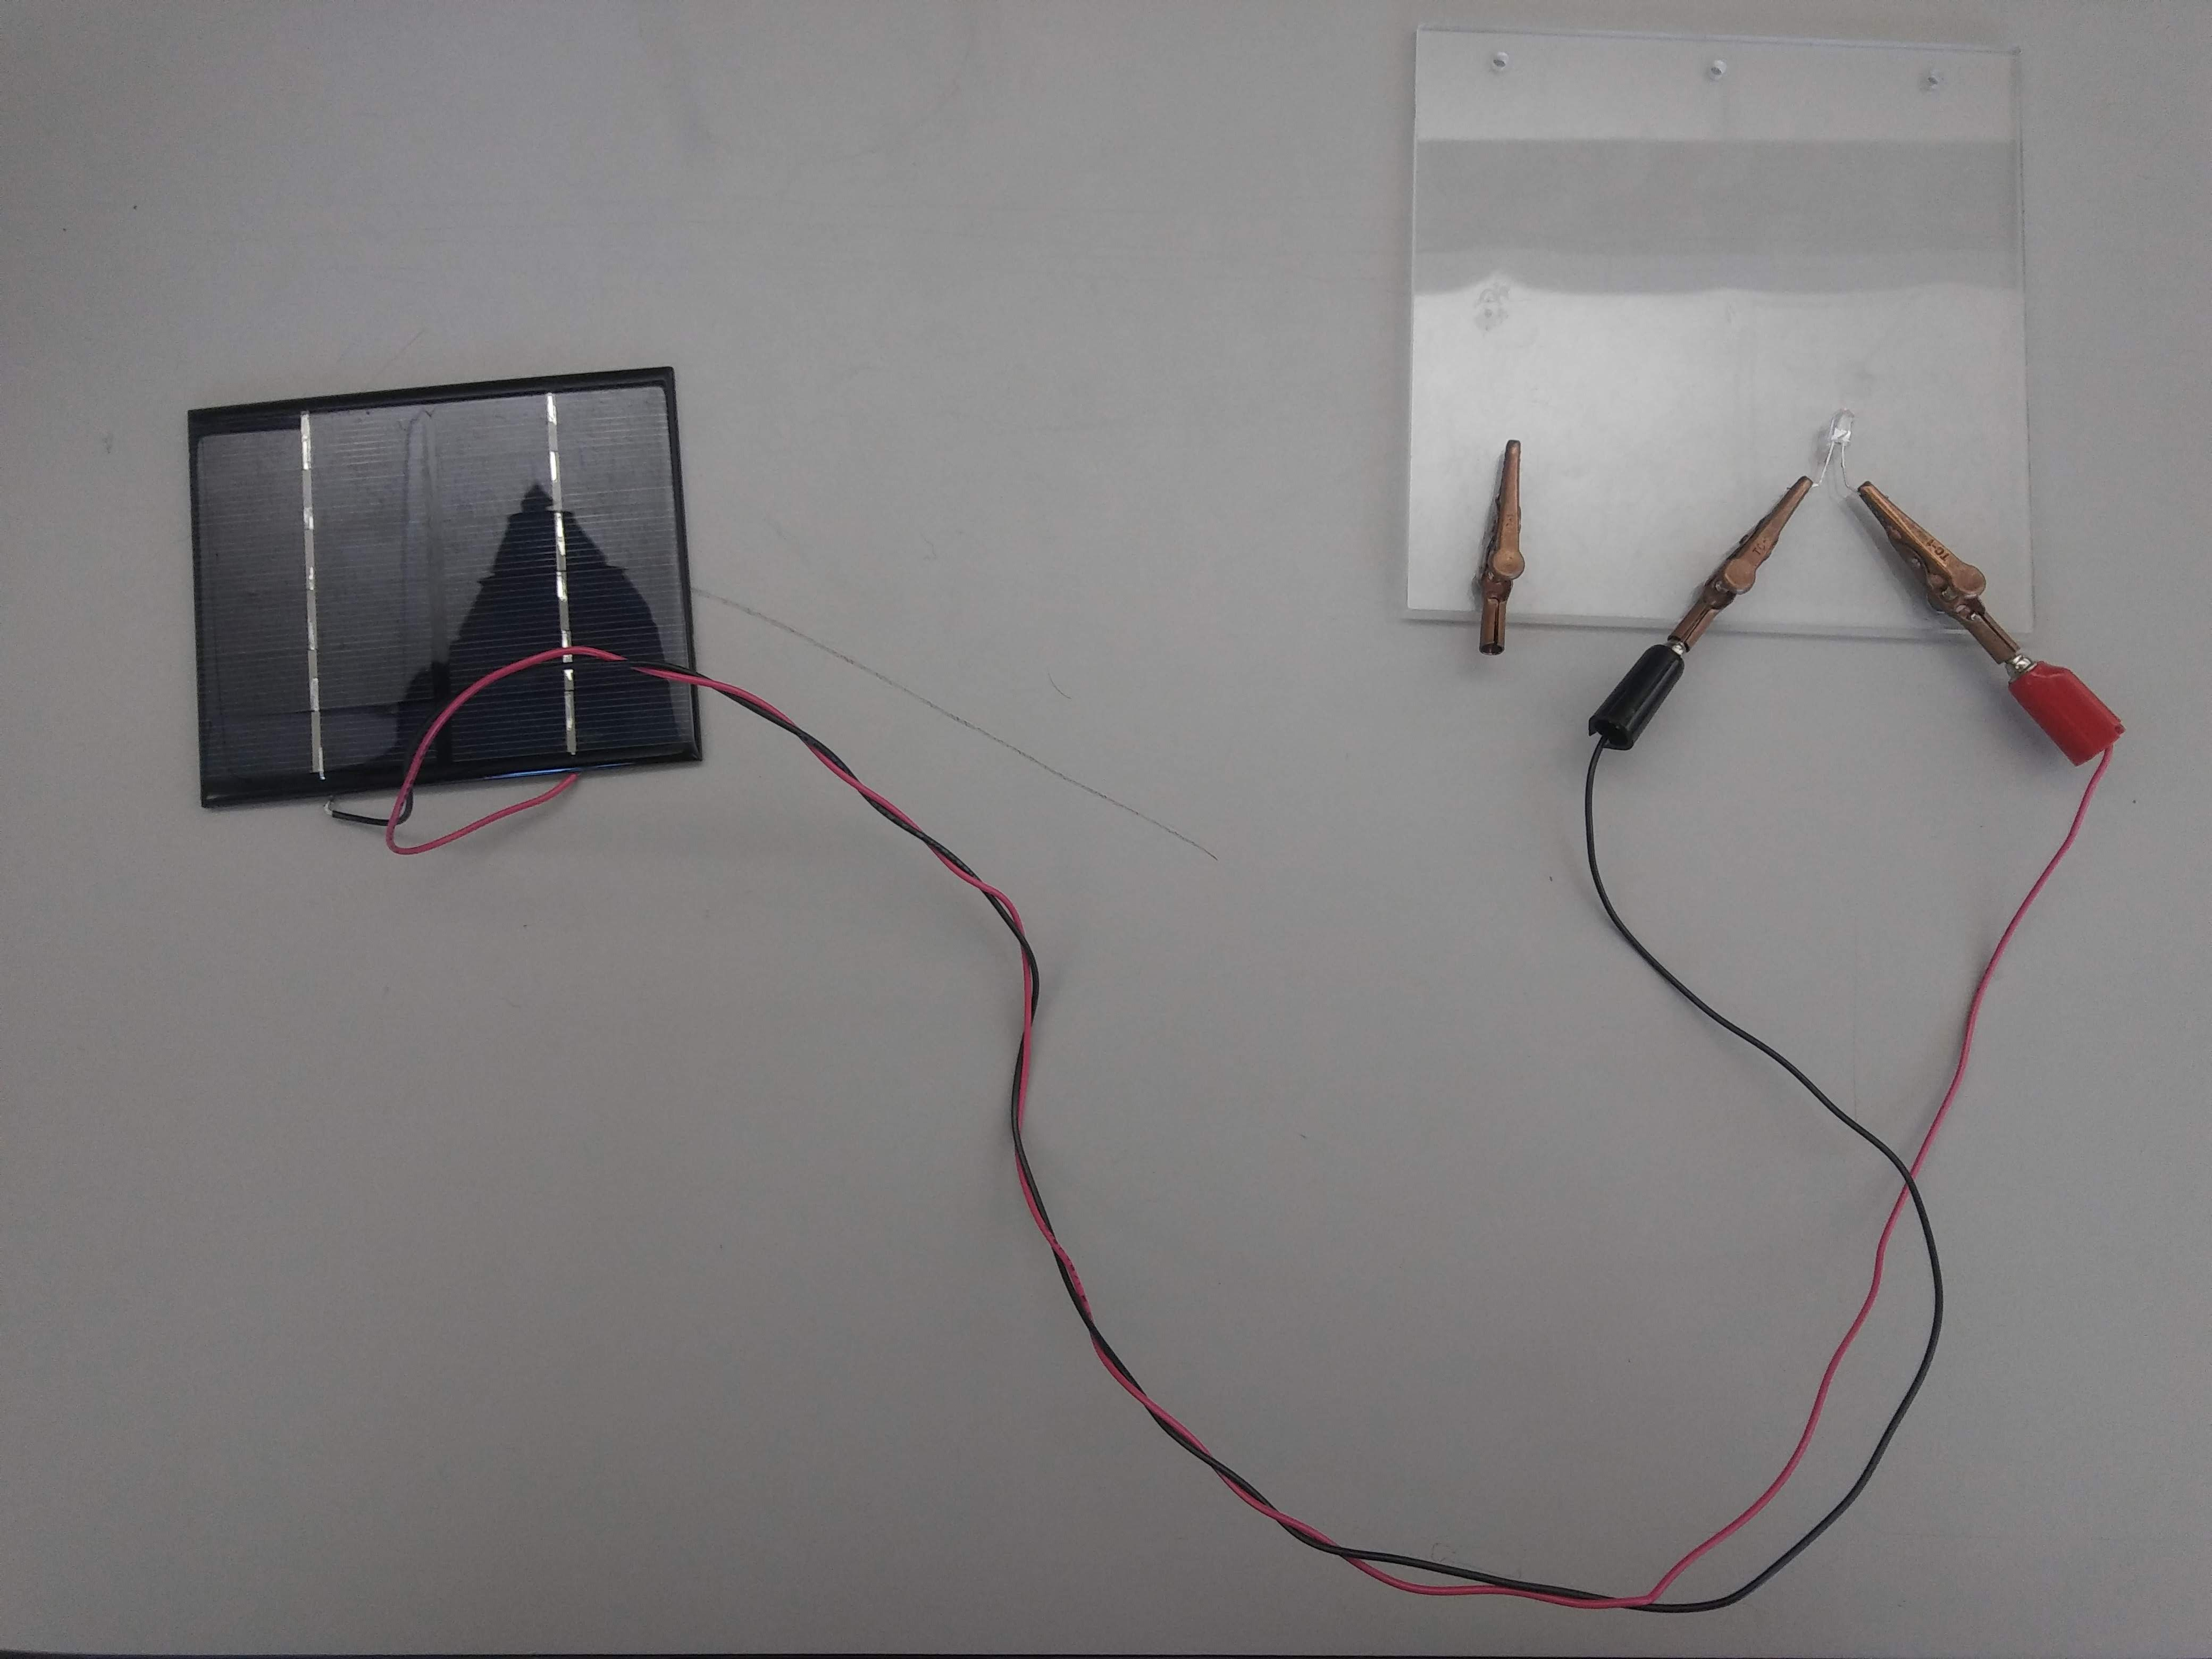
\includegraphics[width=0.7\textwidth]{energy-trans/solar-led}
		\caption{Solar panel connected to the LED.}\label{et:fig:solar-led}
	\end{figure}

Since energy is continuously flowing onto the solar panel and being output from the LED, you will compare the ``power'' instead of the energy. Power is defined as energy per time, so it is how much energy is flowing every second. You can use the last two equations in the Background section to find the input and output power.

\begin{steps}
	\item \textbf{Measure the incoming power.} Turn on the light meter and hold it so that the white dot on top of it is positioned where the solar panel will be. Record the value from the meter. Repeat several times to get an uncertainty.

	\item \textbf{Measure the voltage across the LED.} Ensure that the multimeter is set up to measure voltage (the 'V' setting), one end of the red cable is plugged into the red 'V' socket, and the black cable is plugged into 'COM'. Then plug the other ends of the cables into the two clips attached to the LED. This setup is shown in Fig.\ \ref{et:fig:solar-led-v}. This measures the voltage across the LED, which is like the amount of pressure the solar panel has to apply to get the electrons to go through it.
	
\begin{figure}
	\centering
	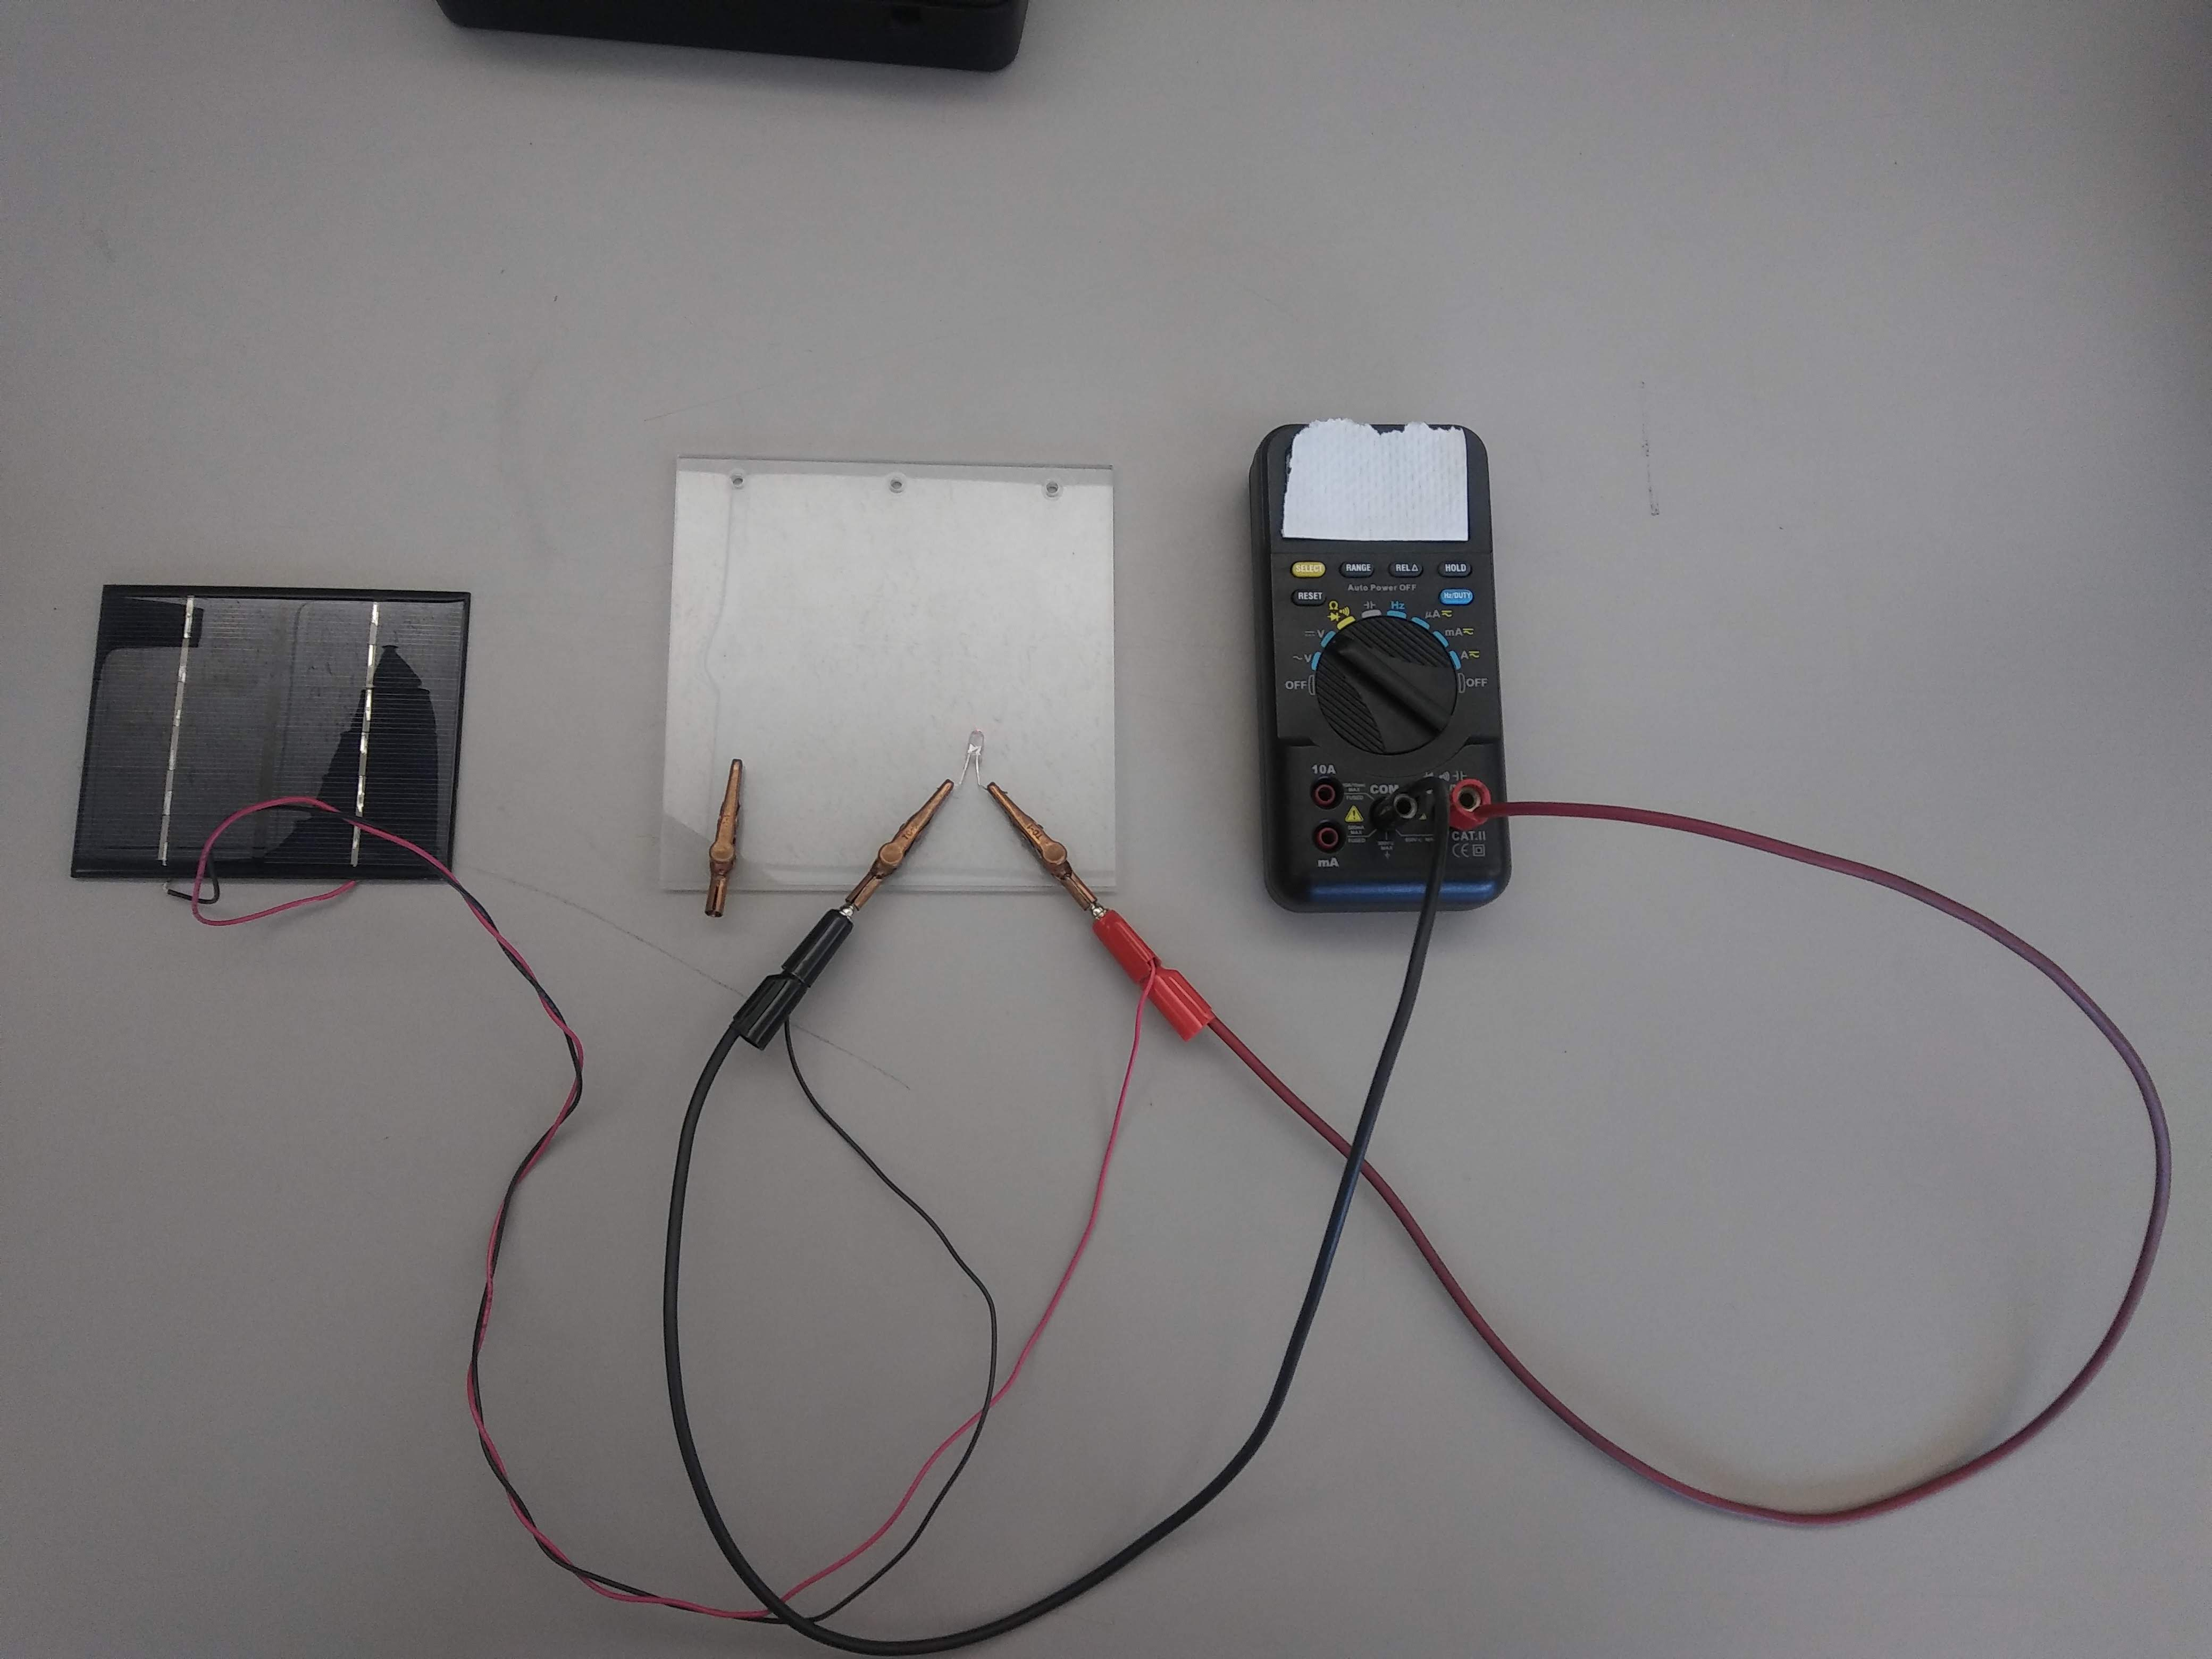
\includegraphics[width=0.7\textwidth]{energy-trans/solar-led-v}
	\caption{Solar panel connected to the LED, with the multimeter attached and set up to measure voltage.}\label{et:fig:solar-led-v}
\end{figure}

	\item \textbf{Measure current through the LED.} Now you will measure the current through the LED. This is a number that is proportional to the number of electrons passing through the wire every second. Ensure that the multimeter is set up to measure current (the `$\mu$A' setting). Then, set up the cables so that the electric current goes from the solar panel's red wire, to the LED, from the other side of the LED to the 'mA' socket on the multimeter, and then from the black 'COM' socket on the multimeter back to the solar panel. This creates a connected loop (circuit) for the electricity to flow through. This setup is described in Figure\ \ref{et:fig:solar-led-ma}. The LED should be lit up when this is correctly set up. \textbf{Record the current reading on the multimeter.}
	
\begin{figure}
	\centering
	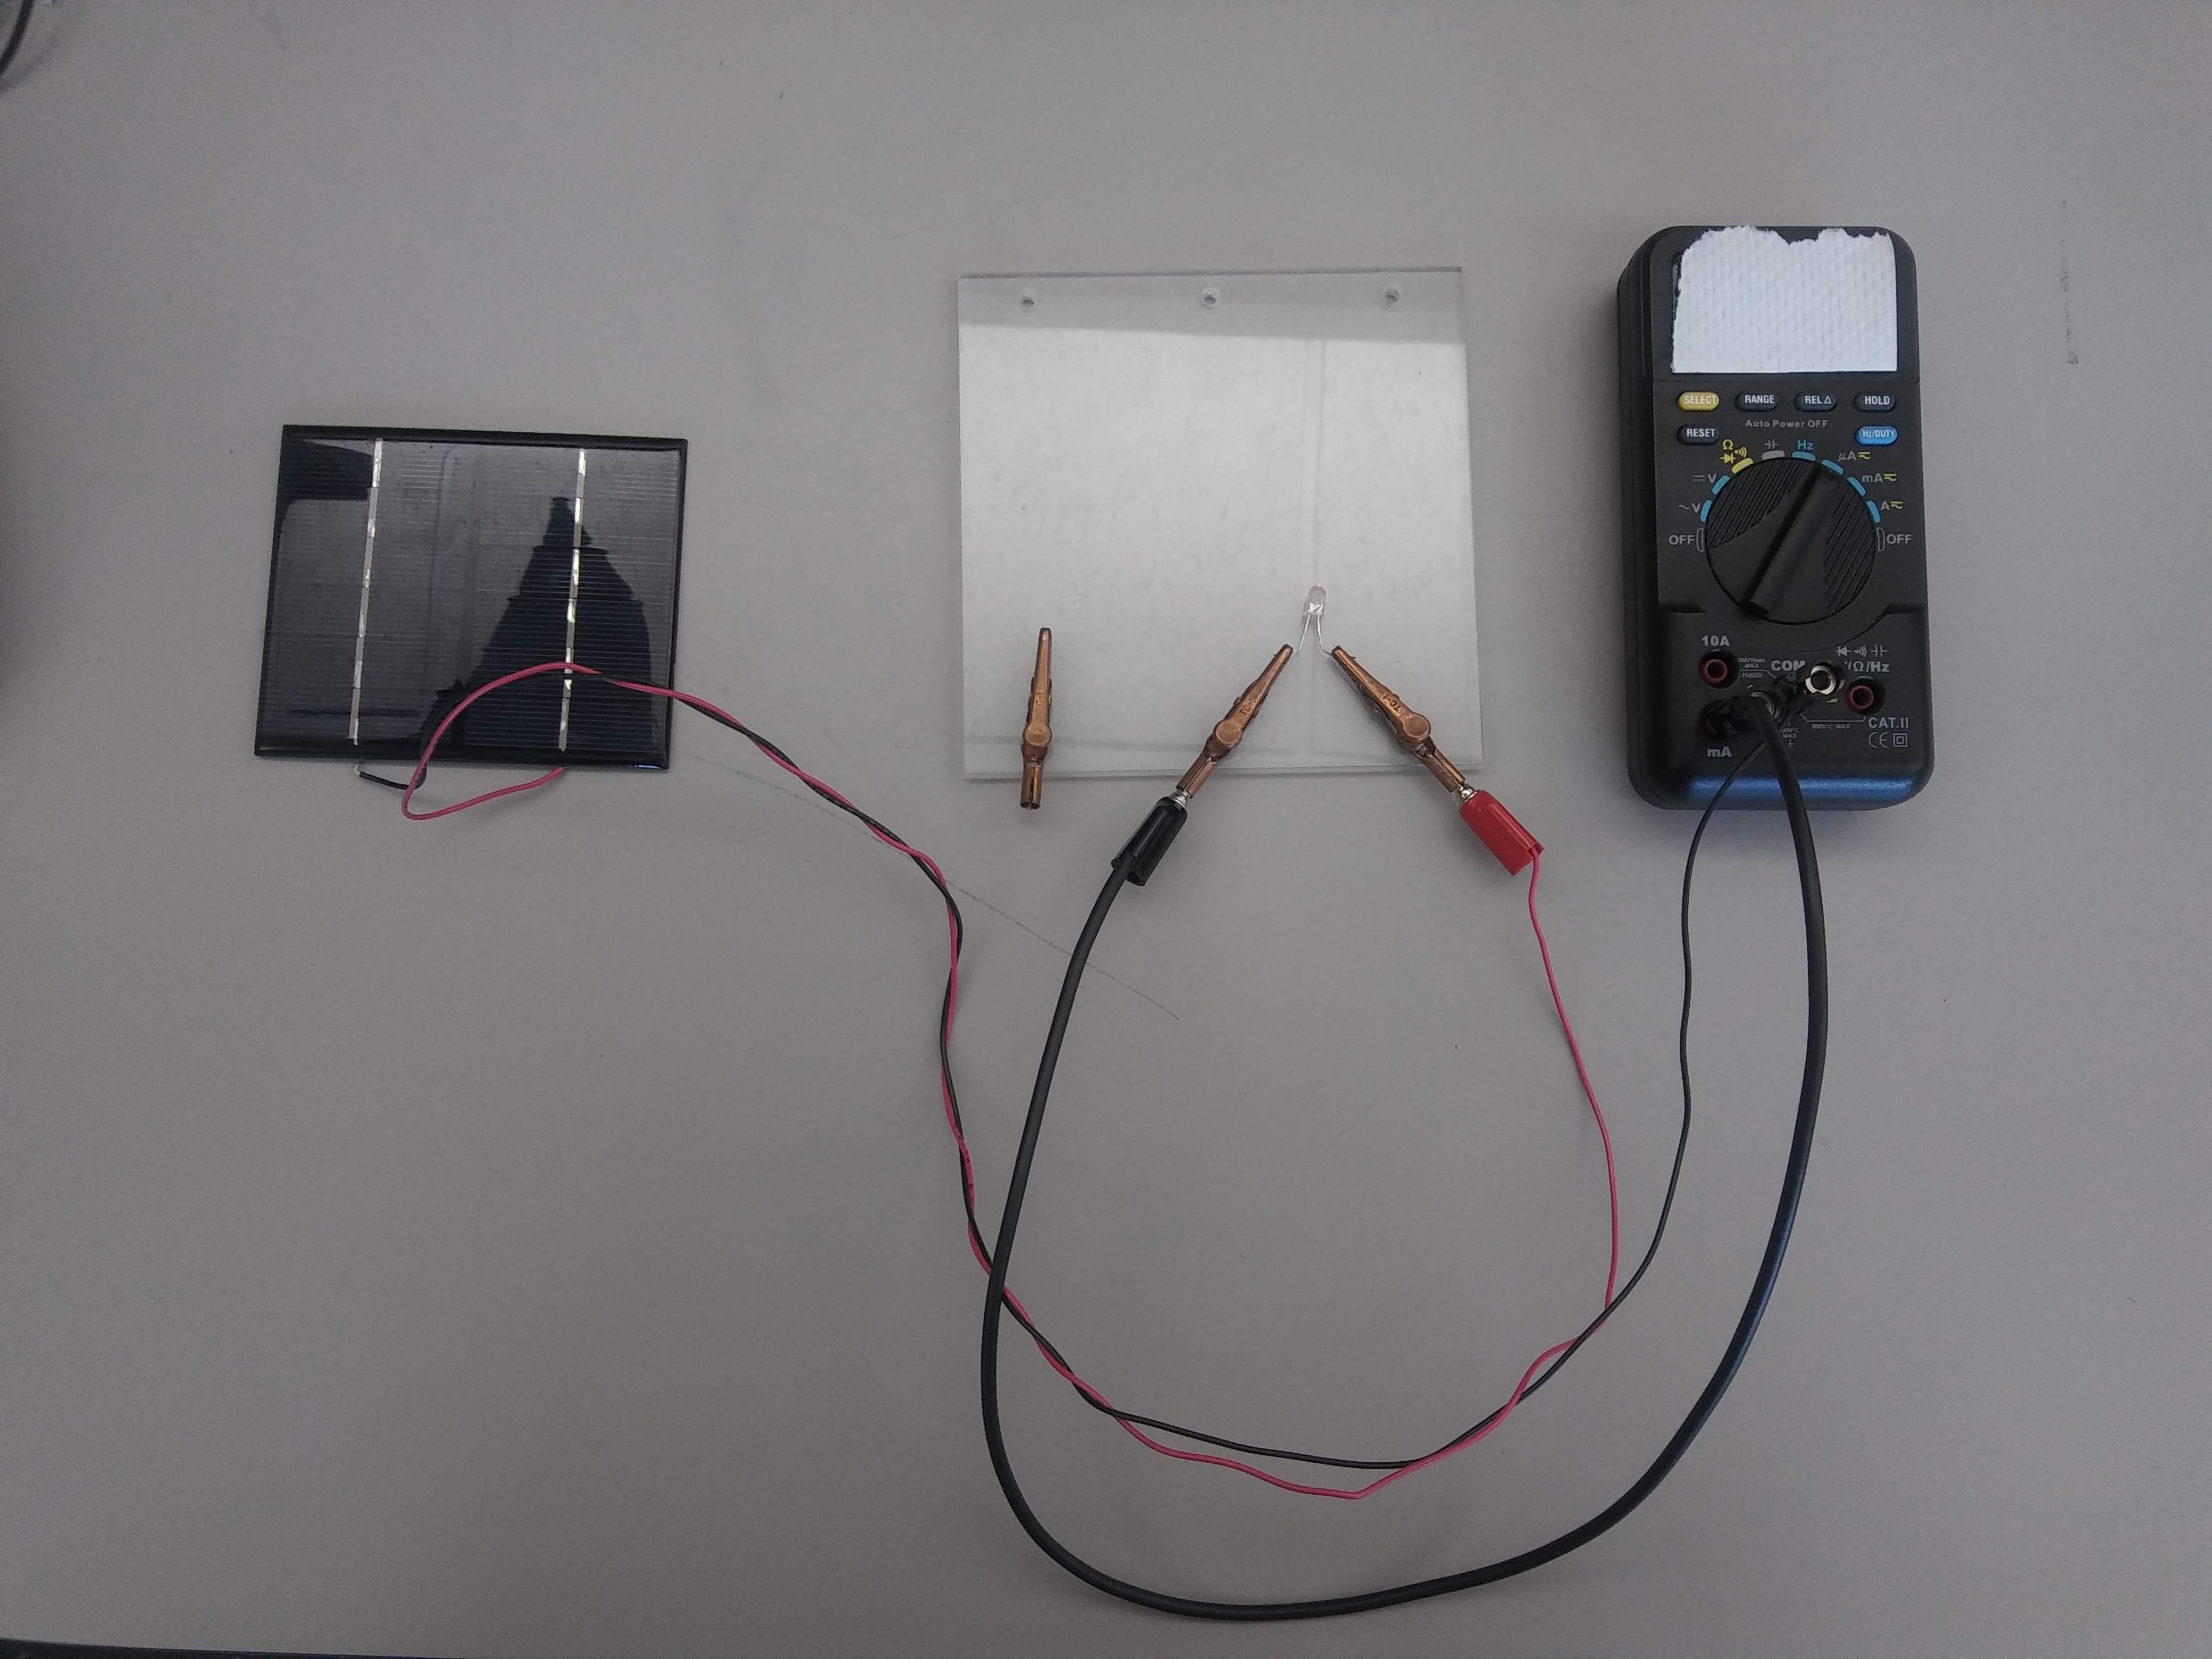
\includegraphics[width=0.7\textwidth]{energy-trans/solar-led-ma}
	\caption{Solar panel connected to the LED, with the multimeter attached and set up to measure current.}\label{et:fig:solar-led-ma}
\end{figure}

	\item Compare the total power input to the solar panel and output through the multimeter. Is it the same, within uncertainties? If not, how do you account for the change? Is there an energy type that you are not measuring? What is that energy type? \textbf{Record your calculations and answers.}
	
	\item In what ways is this similar to light from our sun shining on plants and on water on Earth, and how is it different? \textbf{Record your answers.}
\end{steps}

\section{Report checklist and grading}

Each item below is worth 10 points, and there is an additional 10 points for attendance and participation.

\begin{enumerate}
	\item List of energy transformation history (Step 1).
	
	\item For the car on the ramp: procedure (with sketch of setup), data, analysis, and results including types of energy measured before and after, and amounts of those energies, with uncertainties (Steps 2--4).
	
	\item Car on the ramp: Quantitative comparison of energies before and after, with discussion of extra energy types in play (Step 5).
	
	\item Analogy of car on ramp to star formation (Step 6).
	
	\item Qualitative description of what happened when you pushed down on the fire syringe (Steps 7--8).
	
	\item Analogy of fire syringe to star formation (Step 9).
	
	\item Masses on strings: procedure (with sketch of setup), data, analysis, and results including types of energy measured before and after, and amounts of those energies, with uncertainties (Steps 10--12).
	
	\item Masses on strings: Quantitative comparison of energies before and after, with discussion of extra energy types in play (Step 13).
	
	\item Analogy of masses on strings to black holes merging (Step 14).
	
	\item Data, analysis, and results for the solar panel and LED, including types of energy (per time) measured before and after, and amounts of those energies (per time), with uncertainties (Steps 16--19).
	
	\item Analogy of solar planel to light impinging on Earth (Step 20).
\end{enumerate}
\chapter{Discovering the Hydrogen Atom}

\section{Learning Goals}

\begin{itemize}
	\item Learn to critically evaluate model of physical phenomena and understand how these models are formulated.
	
	\item Develop methods for testing and working with objects which cannot be directly observed. 
	
	\item Gain an understanding of the atomic model and why it differs from what classical physics predicts.
\end{itemize}

\section{Lab Team Roles}

Decide which team members will hold each role this week: facilitator, scribe, technician, skeptic. If there are three members, consider having the skeptic double with another role. Consider taking on a role you are less comfortable with, to gain experience and more comfort in that role.

Additionally, if you are finding the lab roles more restrictive than helpful, you can decide to co-hold some or all roles, or thinking of them more like functions that every team needs to carry out, and then reflecting on how the team executed each function.

\section{Model Evaluation and Construction} %beggingin with these two things, lets see how you can work with these two things

\subsection{Goal} 
When thinking of an atom, we usually tend to imagine a series of electrons orbiting around a nucleus in nice circular orbits. While at first this model might seem unremarkable, the reality is that the physics that describes it is a lot weirder than you think! In order to see why this is, lets see if we can reconstruct the model of the atom qualitatively first. Starting from the assumption that the atom is made up of protons and electrons, over the course of the lab you will create your own model for how these components interact.


\begin{steps} 
	\item First, lets take the classical planetary model of the atom at face value. Using only classical physics concepts, try and find whats wrong with this model. 
	\begin{itemize} 
		\item Think first about what happens to satellites orbiting Earth as they interact with the atmosphere. What forces are acting on it? What happens to it over time?
		
		\item Consider that changing the orbital radius of a body requires a corresponding change in energy. Think about the changes in kinetic and potential energy as the satellite moves closer and farther from the Earth. 
	\end{itemize}
	\item Once your group has come up with an answer, describe what happens to the orbiting object in terms of its energy and its position over time. What implications does this have when you apply it to the atom?
	
	\item After identifying the problem with the model, develop several ideas for a new model which solves the issues you found. \textbf{Forget any previous knowledge of the atom. Think outside the box.} Write down your ideas and describe how they solve the problem. 
	\begin{itemize}
		\item These models don't have to be too complicated, just try thinking of different way in which the electron might move or behave in relation to the nucleus.
	\end{itemize} 
\end{steps}

\section{Observation Experiment: How does an atom absorb and release energy?} %This one should be the assessed experiment. 

\subsubsection{Goal}
Now that you have a rough model of the atom, lets supplement that with some observations to see if you can make it more robust. The difficulty with trying to learn about the structure of the atom is that we have no way of directly observing it. However, we are able to interact with it and observe the results. In this experiment, you will be firing photons at an atom and you will attempt to modify your model based on your observations of the results. 
\subsubsection{Available Equipment}

\begin{itemize}
	\item PHET Models of the Hydrogen Atom Lab: \url{https://phet.colorado.edu/en/simulation/legacy/hydrogen-atom}
\end{itemize}

\subsubsection{Rubrics to be assessed}

B5, B7, B9, C4, C5

\subsubsection{Steps}

\begin{steps} 
	\item Once in the simulation, make sure to turn on the spectrometer, and familiarize yourself with the tools available. Available to you are photon gun which can be set to white or monochromatic (single color) light, a spectrometer which you can take snapshots of, and a speed toggle.
	
	\item To start, try firing white light at the atom. What patterns do you observe? Record any qualitative observations and describe the pattern. 
	
	\item After you have recorded your observations turn off the light, reset the spectrometer, and switch over to monochromatic light. Try firing light of several different wavelengths (colors) at the atom. Record your observations
	
	\item Now, for each of the wavelengths listed, record what happens when photons at that wavelength are fired at the atom. Describe any patterns you observe and include screenshots of the spectrometer. (Try and pay attention to the order in which the photons are emitted)
	\begin{itemize}
		\item Wavelengths to test: 122nm, 103nm, 97nm, 95nm, 94nm 
		
		\item \textbf{Important: Sometimes the simulation might freeze and the atom will appear to no longer emit photons. If that happens, switch over to the white light setting, wait until the atom starts emitting again, switch over to monochromatic light, reset the spectrometer, and continue.}
	\end{itemize}
	
	\item One thing you might have noticed is that for certain wavelengths, the atom might emit several different colors of light. Why might this be happening? Think about it in terms of the energy being absorbed and emitted by the atom. Does it make sense for the atom to be emitting photons at higher wavelengths than the ones absorbed? Remember that energy is inversely proportional to the wavelength of the photon (as one increases the other decreases). Why does the atom absorb at some wavelengths and not others? Record your answers to these questions. 
	
	\item Once you believe you have found a pattern, modify your model of the atom so that it is able to explain these new observations. Record any changes you made and describe how these explain the observed patterns.
	\begin{itemize}
		\item Think about where the energy goes in the atom once its absorbed
		
		\item Does your atom somehow change following an increase in energy? It might help to think back to the classical orbit analogy used int the previous experiment.   
		
		\item How do you account for the fact that only very specific amounts of energy are absorbed and emitted? 
	\end{itemize}

	\item What does your model predict would happen
\end{steps}

\section{Model Evaluation}


\subsection{Available Equipment}

\begin{itemize}
	\item PHET Models of the Hydrogen Atom Lab: \url{https://phet.colorado.edu/en/simulation/legacy/hydrogen-atom}
\end{itemize}

\subsection{The Building Blocks of Everything}
 The word atom finds its roots in the Greek word \textit{atomos} which means indivisible and is believed to have first been used by Democritus to refer to the indivisible spheres which he believed to be the building blocks of our world. Today, we have a far better understanding of the atom and its structure, however, this is information we take for granted. For millennia, there was no clear answer as to what the smallest unit of everything was, and only relatively recently did we develop tools which allowed us to study them more closely. The first comprehensive atomic model was developed in 1803 by John Dalton, who thought of them as solid spheres which changed depending on the element they made up. Then, in 1904, JJ Thompson developed the ``Plum Pudding'' model, which proposed that the atom as made up of electrons floating within a cloud of positive charge. Then in 1911 Ernst Rutherford proposed the nuclear model, where the positive charge was concentrated in the center of the atom. Two years later, Niels Bohr improved upon Thompson's model, suggesting that the orbits were fixed. Finally, Erwin Schrodinger proposed in 1926 the quantum model, where electrons exist around the nucleus in a ``cloud of probability''. You will now have a chance to interact with each of these models.

\subsection{Goal} 
Now that you have developed your own model for what an atom might look like, you will now see the models which at different times were considered the most accurate. You will evaluate each model and try to develop an understanding for the reasoning behind it. 

\subsection{Steps}

\begin{steps}
	\item Make sure the simulation is in ``Prediction'' mode. On the left, you will see a list of all the atomic models organized from ``classical'' to ``quantum''
	
	\item For each model, provide a qualitative description of its structure and behavior. How does it absorb energy? Where does it go once its absorbed? Are there any structural changes? etc. 
	
	\item Along with each description, provide an explanation of the possible reasoning behind each model. What problems does each model address? Why would each model be a good guess as to the structure of an atom. Likewise describe what is wrong with each model. What does it fail to describe or account for?
	
	\item Now compare the model you came up with to some of the other models. Does it resemble any of the other models? Does it improve on some of the shortcomings of the other models? What did you take into account that they did not? Was there anything missing from your model? What did you fail to consider? Write down your observations
	
	\item Along with each description, include a screenshot of the spectrometer for the model. 
	
	\item In the previous experiment, you saw how atoms can only absorb and emit a very specific amount of energy. Provide a rough estimate of the different amounts of energy which the atom is emitting, and if this makes sense given the amount of energy absorbed.
	\begin{itemize}
		\item Use the equation $\mathit{E} = \mathit{h}\nu$ where $\mathit{E}$ is energy joules, $\mathit{h}$ is planck's constant equal to \newline $6.62 \times 10^{-34}$Js, and $\nu$ is the frequency of the emitted photon in hertz.
		
		\item Since you are given the wavelength, use the equation $\nu = \dfrac{c}{\lambda}$ to find the frequency
		
		\item Make sure to include uncertainties in your calculations.
	\end{itemize}
\end{steps}

\section{Group dynamics}

\begin{steps}
	\item Write a 100--200 word reflection on group dynamics and feedback on the lab manual. Address the following topics: who did what in the lab, how did you work together, what successes and challenges in group functioning did you have, and what would you keep and change about the lab write-up?
	
	\item Write a paragraph reporting back from each of the four roles: facilitator, scribe, technician, skeptic. Where did you see each function happening during this lab, and where did you see gaps?
\end{steps}

\section{Report checklist and grading}

The lab grade consists of 3 points for each of seven scientific ability rubric rows (the 5 listed above, which apply just to that section, as well as F1 and F2, applied to the entire report), and 9 points for providing evidence in the lab report of completing all steps of the lab, including answering every question, for a total of 30 points.

\appendix

\chapter{Analysis of Uncertainty}

A physical quantity consists of a value, unit, and uncertainty.
For example, ``$5 \pm 1\,$m'' means that the writer believes the true value of the quantity to most likely lie within 4 and 6 meters\footnote{The phrase ``most likely'' can mean different things depending on who is writing.
	If a physicist gives the value and does not given a further explanation, we can assume that they mean that the measurements are randomly distributed according to a normal distribution around the value given, with a standard deviation of the uncertainty given.
	So if one were to make the same measurement again, the author believes it has a 68\% chance of falling within the range given.
	Disciplines other than physics may intend the uncertainty to be 2 standard deviations.}.
Without knowing the uncertainty of a value, the quantity is next to useless.
For example, in our daily lives, we use an implied uncertainty.
If I say that we should meet at around 5:00 pm, and I arrive at 5:05 pm, you will probably consider that within the range that you would expect.
Perhaps your implied uncertainty is plus or minus 15 minutes.
On the other hand, if I said that we would meet at 5:07 pm, then if I arrive at 5:10 pm, you might be confused, since the implied uncertainty of that time value is more like 1 minute.

Scientists use the mathematics of probability and statistics, along with some intuition, to be precise and clear when talking about uncertainty, and it is vital to understand and report the uncertainty of quantitative results that we present.

\section{Types of measurement uncertainty}

For simplicity, we limit ourselves to the consideration of two types of uncertainty in this lab course, instrumental and random uncertainty.

\subsection{Instrumental uncertainties}

Every measuring instrument has an inherent uncertainty that is determined by the precision	
  of the instrument.
Usually this value is taken as a half of the smallest increment of the instrument's scale. For example, $0.5\:$mm is the precision of a standard metric ruler; $0.5\:$s is the precision of a watch, etc. For electronic digital displays, the equipment's manual often gives the instrument's resolution, which may be larger than that given by the rule above.

Instrumental uncertainties are the easiest ones to estimate, but they are not the only source of the uncertainty in your measured value.
You must be a skillful experimentalist to get rid of all other sources of uncertainty so that all that is left is instrumental uncertainty.

\subsection{Random uncertainties}

Very often when you measure the same physical quantity multiple times, you can get different results each time you measure it.
That happens because different uncontrollable factors affect your results randomly.
This type of uncertainty, random uncertainty, can be estimated only by repeating the same measurement several times.
For example if you measure the distance from a cannon to the place where the fired cannonball hits the ground, you could get different distances every time you repeat the same experiment.	
  
For example, say you took three measurements and obtained 55.7, 49.0, 52.5, 42.4, and 60.2 meters. We can quantify the variation in these measurements by finding their standard deviation using a calculator, spreadsheet, or the formula (assuming the data distributed according to a normal distribution)
\begin{equation}
 \sigma = \sqrt{\sum_{i=1}^{N} \frac{(x_i-\bar{x})^2}{N-1}} \, ,
\end{equation}
where $\{x_1, x_2, \dots, x_N\}$ are the measured values, $\bar{x}$ is the mean of those values, and $N$ is the number of measurements.
For our example, the resulting standard deviation is 6.8 meters. Generally we are interested not in the variation of the measurements themselves, but how uncertain we are of the average of the measurements. The uncertainty of this mean value is given, for a normal distribution, by the so-called ``standard deviation of the mean'', which can be found by dividing the standard deviation by the square root of the number of measurements,
\begin{equation}
\sigma_\textrm{mean} = \frac{\sigma}{\sqrt{N}} \, .
\end{equation}
So, in this example, the uncertainty of the mean is 3.0 meters. We can thus report the length as $52 \pm 3\:$m.

Note that if we take more measurements, the standard deviation of those measurements will not generally change, since the variability of our measurements shouldn't change over time. However, the standard deviation of the mean, and thus the uncertainty, will decrease.

\section{Propagation of uncertainty}

When we use an uncertain quantity in a calculation, the result is also uncertain. To determine by how much, we give some simple rules for basic calculations, and then a more general rule for use with any calculation which requires knowledge of calculus. Note that these rules are strictly valid only for values that are normally distributed, though for the purpose of this course, we will use these formulas regardless of the underlying distributions, unless otherwise stated, for simplicity.

If the measurements are completely independent of each other, then for quantities $a \pm \delta a$ and $b \pm \delta b$, we can use the following formulas:
\begin{equation}\label{unc:add}
\textrm{For } c = a + b \textrm{ (or for subtraction), } \delta c = \sqrt{(\delta a)^2 + (\delta b)^2}
\end{equation}

\begin{equation}\label{unc:mult}
\textrm{For } c = ab \textrm{ (or for division), } \frac{\delta c}{c} = \sqrt{\left(\frac{\delta a}{a}\right)^2 + \left(\frac{\delta b}{b}\right)^2}
\end{equation}

\begin{equation}\label{unc:exp}
\textrm{For } c = a^n,\, \frac{\delta c}{c} = n \frac{\delta a}{a}
\end{equation}

If you are familiar with calculus, you may want to use this general formula for the uncertainty $\delta f$ of a function $f$ of $N$ independent values $x_i$, each with uncertainty $\delta x_i$:
\begin{equation}\label{unc:general}
\delta f = \sqrt{ \sum_{i=1}^{N} \left(\frac{\partial f}{\partial x_i} \delta x_i\right)^2 } \, .
\end{equation}
Notice that Eqs.\ \ref{unc:add} through \ref{unc:exp} can be derived from Eq.\ \ref{unc:general} for those specific cases.

\subsubsection{What if there is no reported uncertainty?}

Sometimes you'll be calculating with numbers that have no uncertainty given.
In some cases, the number is exact.
For example, the circumference $C$ of a circle is given by $C = 2 \pi r$. Here, the coefficient, $2\pi$, is an exact quantity and you can treat its uncertainty as zero.
If you find a value that you think is uncertain, but the uncertainty is not given, a good rule of thumb is to assume that the uncertainty is half the right-most significant digit.
So if you are given a measured length of $1400\:$m, then you might assume that the uncertainty is $50\:$m.
This is an assumption, however, and should be described as such in your lab report.
For more examples, see Table~\ref{unc:tab:implied}.

\begin{table}
	\begin{center}
		\begin{tabular}{cc}
			\textbf{Expression} & \textbf{Implied uncertainty} \\
			12 & 0.5 \\
			12.0 & 0.05 \\
			120 & 5 \\
			120. & 0.5
		\end{tabular}
		\caption{Expression of numbers and their implied uncertainty.}\label{unc:tab:implied}
	\end{center}
\end{table}

\subsubsection{How many digits to report?}

After even a single calculation, a calculator will often give ten or more digits in an answer.
For example, if I travel $11.3 \pm 0.1\:$km in $350 \pm 10\:$s, then my average speed will be the distance divided by the duration. Entering this into my calculator, I get the resulting value ``\texttt{0.0322857142857143}''.
Perhaps it is obvious that my distance and duration measurements were not precise enough for all of those digits to be useful information.
We can use the propagated uncertainty to decide how many decimals to include.
Using the formulas above, I find that the uncertainty in the speed is given by my calculator as ``\texttt{9.65683578099600e-04}'', where the `\texttt{e}' stands for ``times ten to the''.
I definitely do not know my uncertainty to 14 decimal places.
For reporting uncertainties, it general suffices to use just the 1 or 2 left-most significant digits, unless you have a more sophisticated method of quantifying your uncertainties.
So here, I would round this to 1 significant digit, resulting in an uncertainty of $0.001\:$km/s.
Now I have a guide for how many digits to report in my value.
Any decimal places to the right of the one given in the uncertainty are distinctly unhelpful, so I report my average speed as ``$0.032 \pm 0.001\:$km/s''.
You may also see the equivalent, more succinct notation ``$0.032(1)\:$km/s''.

\section{Comparing two values}\label{unc:sec:comparing}

If we compare two quantities and want to find out how different they are from each other, we can use a measure we call a $t'$ value (pronounced ``tee prime''). This measure is not a standard statistical measure, but it is simple and its meaning is clear for us.

Operationally, for two quantities having the same unit, $a \pm \delta a$ and $b \pm \delta b$, the measure is defined as\footnote{Statistically, if $\delta a$ and $\delta b$ are uncorrelated, random uncertainties, then $t'$ represents how many standard deviations the difference $a - b$ is away from zero.}

\begin{equation}
%t' = \frac{\abs{a-b}}{\sqrt{(\delta a)^2 + (\delta b)^2}}
t' = \frac{\abs{a-b}}{\sqrt{(\delta a)^2 + (\delta b)^2}}
\end{equation}

If $t' \lesssim 1$, then the values are so close to each other that they are indistinguishable. It is either that they represent the same true value, or that the measurement should be improved to reduce the uncertainty.

If $1 \lesssim t' \lesssim 3$, then the result is inconclusive. One should improve the experiment to reduce the uncertainty.

If $t' \gtrsim 3$, then the true values are very probably different from each other.
\begin{landscape}
\chapter{Rubrics}
	
	\freetabcaption{Rubric B: Ability to design and conduct an observational experiment \cite{etkina_scientific_2006}.}
	\begin{longtable}{>{\bfseries}p{0.02\textheight}|>{\bfseries\RaggedRight}p{0.25\textheight}|>{\RaggedRight}p{0.21\textheight}|>{\RaggedRight}p{0.21\textheight}|>{\RaggedRight}p{0.22\textheight}|>{\RaggedRight}p{0.22\textheight}}
		\toprule
		& Scientific Ability
		& Missing & Inadequate & Needs Improvement & Adequate \\ \midrule \endhead
		B1
		& Is able to identify the phenomenon to be investigated
		& No phenomenon is mentioned
		& The description of the phenomenon to be investigated is confusing, or it is not the phenomenon of interest.
		& \midsloppy The description of the phenomenon is vague or incomplete.
		& The phenomenon to be investigated is clearly stated. \\ \midrule
		B2
		& Is able to design a reliable experiment that investigates the phenomenon
		& The experiment does not investigate the phenomenon.
		& The experiment may not yield any interesting patterns.
		& Some important aspects of the phenomenon will not be observable.
		& The experiment might yield interesting patterns relevant to the investigation of the phenomenon. \\ \midrule
		B3
		& Is able to decide what physical quantities are to be measured and identify independent and dependent variables
		& The physical quantities are irrelevant.
		& Only some of physical quantities are relevant.
		& The physical quantities are relevant. However, independent and dependent variables are not identified.
		& The physical quantities are relevant and independent and dependent variables are identified. \\ \midrule
		B4
		& Is able to describe how to use available equipment to make measurements
		& At least one of the chosen measurements cannot be made with the available equipment.
		& All chosen measurements can be made, but no details are given about how it is done.
		& All chosen measurements can be made, but the details of how it is done are vague or incomplete.
		& All chosen measurements can be made and all details of how it is done are clearly provided. \\ \midrule
		B5
		& Is able to describe what is observed without trying to explain, both in words and by means of a picture of the experimental setup.
		& No description is mentioned.
		& A description is incomplete. No labeled sketch is present. Or, observations are adjusted to fit expectations.
		& A description is complete, but mixed up with explanations or pattern. Or the sketch is present but is difficult to understand.
		& Clearly describes what happens in the experiments both verbally and with a sketch. Provides other representations when necessary (tables and graphs). \\ \midrule
		B6
		& Is able to identify the shortcomings in an experiment and suggest improvements
		& No attempt is made to identify any shortcomings of the experiment.
		& The shortcomings are described vaguely and no suggestions for improvement are made.
		& Not all aspects of the design are considered in terms of shortcomings or improvements.
		& All major shortcomings of the experiment are identified and reasonable suggestions for improvement are made. \\ \midrule
		B7
		& Is able to identify a pattern in the data
		& No attempt is made to search for a pattern.
		& The pattern described is irrelevant or inconsistent with the data.
		& The pattern has minor errors or omissions. Terms like ``proportional'' used without clarity, e.g.\ is the proportionality linear, quadratic, etc.
		& The pattern represents the relevant trend in the data. When possible, the trend is described in words. \\ \midrule
		B8
		& Is able to represent a pattern mathematically (if applicable)
		& No attempt is made to represent a pattern mathematically.
		& The mathematical expression does not represent the trend.
		& No analysis of how well the expression agrees with the data is included, or some features of the pattern are missing.
		& The expression represents the trend completely and an analysis of how well it agrees with the data is included. \\ \midrule
		B9
		& Is able to devise an explanation for an observed pattern
		& No attempt is made to explain the observed pattern.
		& An explanation is vague, not testable, or contradicts the pattern.
		& An explanation contradicts previous knowledge or the reasoning is flawed.
		& A reasonable explanation is made. It is testable and it explains the observed pattern. \\
		\bottomrule
	\end{longtable}

	
%\end{table}

\end{landscape}
% This format is not a formal report, but simply answering questions, including figures, and demonstrating scientific abilities.
\chapter{Lab Report Format}\label{cha:lab-report-format}

%TODO Make firm page limit? 5 pages + figures and tables?

%In a general sense, the labs should demonstrate the rubric rows listed in the lab write-up and provide answers to every lab question asked.

\section{General}

\begin{itemize}
	\item The report should be typed for ease of reading. Text should be double-spaced, and the page margins (including headers and footers) should be approximately $2.5\:$cm, for ease of marking by the grader. Each page should be numbered.
	
	\item The first page should include the title of the lab; lab section day, time, and number; and the names of the members of your lab team.
	
%	\item If the rubric row refers to a particular part of your lab report, clearly label that part of the report with that rubric row. For example, you should label the section where you demonstrate uncertainty propagation with ``G2'' if that rubric row is being assessed in that lab.
\end{itemize}

\section{Organizing the report}

%If the lab is clearly framed as an observational, testing, or application experiment, you can follow the corresponding rubric for the elements to include in the report (see, respectively, Rubrics B, C, and D in Appendix~\ref{cha:rubrics}).

The report should follow the sequence of the report checklist. Answers to questions and inclusion of tables and figures should appear in the order they are referenced in the manual. In general, include the following:

	\begin{itemize}
%		\item Any procedure that you performed that is different from what is described in the lab manual.
		
%		\item Any data that you've collected: tables, figures, measured values, sketches. Whenever possible, include an estimate of the uncertainty of measured values.
		
		\item For any calculations that you perform using your data, and the final results of your calculation, you must show your work in order to demonstrate to the grader that you have actually done it. Even if you're just plugging numbers into an equation, you should write down the equation and all the values that go into it. This includes calculating uncertainty and propagation of uncertainty.
		
		\item If you are using software to perform a calculation, you should explicitly record what you've done. For example, ``Using Excel we fit a straight line to the velocity vs. time graph. The resulting equation is $v = (0.92\:\mathrm{m/s^2}) t + 0.2\:\mathrm{m/s}$.''
		
		\item Answers to any questions that appear in the lab handout. Each answer requires providing justification for your answer.
		
%		\item At the end of each experiment, you should discuss the findings and reflect deeply on the quality and importance of the findings%
		% (Rubric Row F2)
%		. This can be both in the frame of a scientist conducting the experiment (``What did the experiment tell us about the world?'') and in the frame of a student (``What skills or mindsets did I learn?'').
	\end{itemize}

\section{Graphs, Tables, and Figures}

Any graph, table, or figure (a figure is any graphic, for example a sketch) should include a caption describing what it is about and what features are important, or any helpful orientation to it. The reader should be able to understand the basics of what a graph, table, or figure is saying and why it is important without referring to the text. For more examples, see any such element in this lab manual.

Each of these elements has some particular conventions.

\subsection{Tables}

A table is a way to represent tabular data in a quantitative, precise form. Each column in the table should have a heading that describes the quantity name and the unit abbreviation in parentheses. For example, if you are reporting distance in parsecs, then the column heading should be something like ``distance (pc)''. This way, when reporting the distance itself in the column, you do not need to list the unit with every number.

\subsection{Graphs}

A graph is a visual way of representing data. It is helpful for communicating a visual summary of the data and any patterns that are found.

The following are necessary elements of a graph of two-dimensional data (for example, distance vs. time, or current vs. voltage) presented in a scatter plot.

\begin{itemize}
	\item \textbf{Proper axes.} The conventional way of reading a graph is to see how the variable on the vertical axis changes when the variable on the horizontal axis changes. If there are independent and dependent variables, then the independent variable should be along the horizontal axis.
	
	\item \textbf{Axis labels.} The axes should each be labeled with the quantity name and the unit abbreviation in parentheses. For example, if you are plotting distance in parsecs, then the axis label should be something like ``distance (pc)''.
	
	\item \textbf{Uncertainty bars.} If any quantities have an uncertainty, then these should be represented with so-called ``error bars'', along both axes if present. If the uncertainties are smaller than the symbol used for the data points, then this should be explained in the caption.

\end{itemize}

%\include{scidavis/scidavis}

% \bibliography{references,MyLibrary}
% \bibliographystyle{plain}
\printbibliography

\end{document}
